\documentclass[11pt,twoside,final]{memoir}

\usepackage{mylayout}

%% Details of the book
%% ===================

\title{Consapevolezza: la via al senza-morte}
\subtitle{Insegnamenti sulla meditazione del Venerabile Ajahn Sumedho}
\author{Ajahn Sumedho}
\date{}
\editionInfo{}
% Title comment: ...
% Publisher name: ...
% Printer name: ...
\ISBN{978-8-8885706-35-4}
% Copyright text: ...

%% Load further packages
%% =====================

% \usepackage{lipsum}

%% Hyphenation exceptions and corrections
%% ======================================

\hyphenation{dhamma}

\begin{document}

%\emptysheet

%% Frontmatter
%% ===========

\frontmatter*
\midsloppy

%% About
%% -----
%% Short review or summary of the book, or comments by others.
%% Brief bigraphy of the author, translator, editor, and their connection to the text.

\cleartoverso
\thispagestyle{empty}

{\centering\par
\Large\scshape\chapTitleFont\thetitle
\par}
\vspace*{2\baselineskip}

{%
\setlength{\parskip}{1.5em}
\setlength{\parindent}{0pt}

Il materiale di questo libro è tratto da discorsi tenuti al monastero della Foresta di Chithurst (Regno Unito) nel Gennaio 1984, con l'eccezione dei capitoli ``\textit{Sforzo e rilassamento},'' ``\textit{Benevolenza}'' e ``\textit{Gli impedimenti e la cessazione degli impedimenti},'' che sono estratti da discorsi dati nel Dicembre del 1982 al monastero Internazionale della Foresta (Wat Pah Nanachat) di Ubon, nel nord-est della Thailandia.

% The photographs are of slabs from the ruins of the ancient \textit{stūpa} at Amaravati in Andhra Pradesh, India; they are reproduced by kind permission of the Trustees of the British Museum, London.
%
% Page \pageref{image-stupa}: the \textit{stūpa}, a monumental reliquary, contains the relics of a saint. As the object of pilgrimages, it symbolizes the universal quest for spiritual truth.
%
% Page \pageref{image-feet}: the iconographical footprints of the Buddha. They represent the path that a teacher has taken, to be followed by his disciples.
%
% Page \pageref{image-lotus-scene}: the lotus of wisdom in a scene of everyday human activity.
%
% Le fotografie mostrano lastre delle rovine dell'antico stupa di Amaravati in Andhra Pradesh, in India. Sono riprodotte su gentile concessione dell'amministrazione del British Museum di Londra.
%
% Pagina 22: lo stupa, un imponente reliquiario, contiene le reliquie di un santo. Come luogo di pellegrinaggio, simboleggia l'universale ricerca della verità spirituale.
%
% Pagina 36: le orme iconografiche del Buddha. Rappresentano il sentiero che l'insegnante ha intrapreso, e che sarà seguito dai discepoli.
%
% Pagina 100: il loto della saggezza in una scena quotidiana di vita umana.

\clearpage
\thispagestyle{empty}

{\scshape \theauthor} è nato negli USA, a Seattle nel 1934. Ha preso l'ordinazione come bhikkhu (monaco della tradizione Theravāda) in Thailandia nel 1966 e ha trascorso dieci anni nel nord-est del Paese con il Venerabile Ajahn Chah, insegnante della tradizione spirituale dei ``Maestri della Foresta.'' Invitato nel 1976 in Inghilterra da un'associazione laica (English Sangha Trust) ha successivamente fondato i monasteri di Chithurst e di Amaravati in Inghilterra, inoltre ha incoraggiato e sostenuto l'apertura di altri monasteri, fra cui il Santacittarama in Italia, contribuendo a diffondere la tradizione Theravāda in diversi paesi occidentali. Nel 2010, dopo 33 anni di servizio nelle comunità occidentali, ha deciso di lasciare i suoi incarichi pubblici e ritornare in Thailandia per continuare la sua vita monastica in forma più ritirata. Negli ultimi anni si è trasferito nuovamente in Inghilterra dove risiede al monastero di Amaravati.

{\scshape Ajahn Sucitto} è stato l'abate di Cittaviveka, monastero buddhista di Chithurst, dal 1992. Nel 1986 ha offerto il suo contributo a questo libretto, scrivendone la prefazione. È nato a Londra nel 1949. Nel Marzo 1976 venne ordinato bhikkhu in Thailandia. Ritornò in Gran Bretagna nel 1978 dove incominciò la sua formazione con Ajahn Sumedho al vihara buddhista di Hampstead, a Londra. Nel 1979 fece parte del piccolo gruppo storico di monaci che, con Ajahn Sumedho, fondò Cittaviveka, il monastero buddhista di Chithurst, nel West Sussex. Attualmente vive ancora a Cittaviveka, ma ha lasciato il ruolo di abate per dedicarsi maggiormente all'insegnamento.

}



%% Title page
%% ----------
%% subtitle, editor, translator, preface by, introduction by, publisher

\cleartorecto
\thispagestyle{empty}

\vspace*{5em}

{\centering

{\Large\chapTitleFont\scshape\thetitle}
\medskip

{\itshape\thesubtitle}
\vspace*{220pt}


{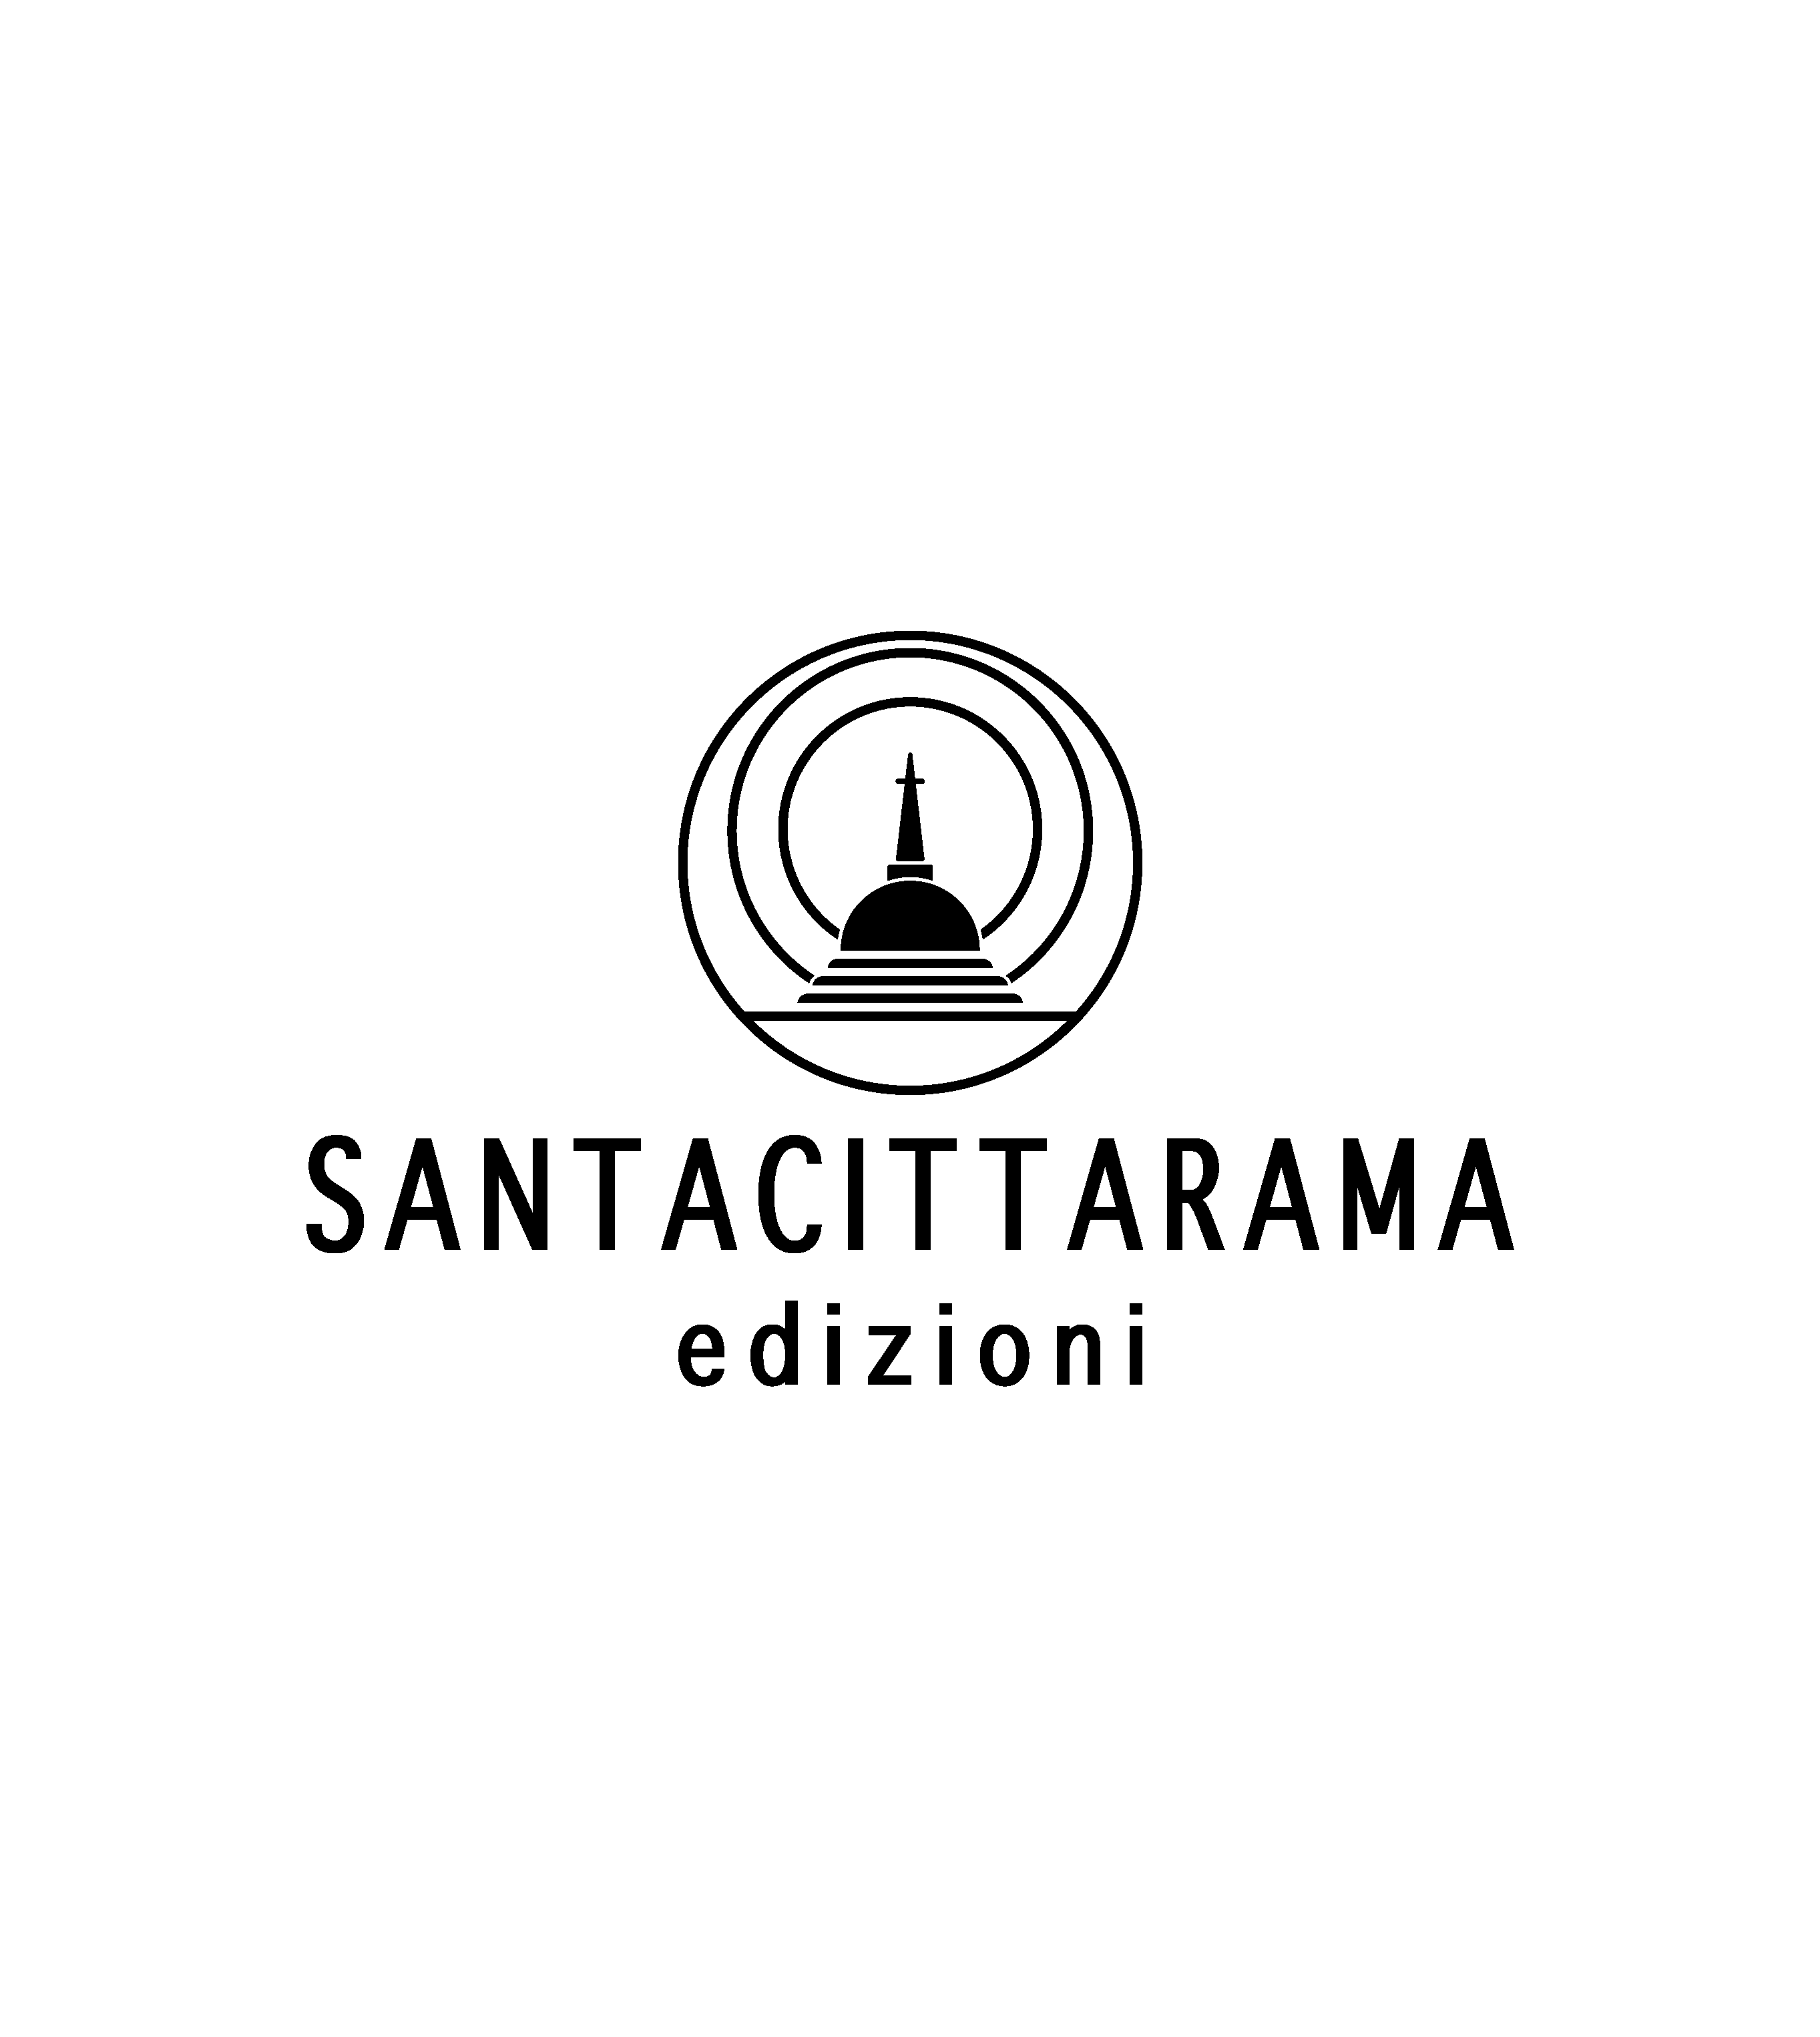
\includegraphics[height=35mm,keepaspectratio,]{logo.png}}

% \theauthor

}


%% Copyright page
%% --------------
%% publisher info, edition info, ISBN, etc.

\cleartoverso
\thispagestyle{empty}
{\small\setlength{\parskip}{0.8em}\setlength{\parindent}{0em}%
{\raggedright%

\enlargethispage*{\baselineskip}

\thetitle\\
di \theauthor

Pubblicato da:\\
Edizioni Santacittarama,\\
Monastero Santacittarama,\\
Località Brulla snc\\
02030 Poggio Nativo (RI), \\
Italia

Questo libro è scaricabile gratuitamente all’indirizzo\\
www.santacittarama.org e www.fsbooks.org

Traduzione di Letizia Baglioni

ISBN \theISBN

Copyright \copyright\ 2022 Associazione Santacittarama

%\copyright\ Associazione Santacittarama, 2012. Tutti i diritti sono riservarti.

Titolo originale: Mindfulness: The Path to the Deathless\\
\copyright\ Amaravati Publications, 1985

% Foto copertina di ...

\vfill

\raggedright
2012, 2.000 copie, stampate in Malesia\\
2017, 2.000 copie, stampate in Malesia\\
2022, 3.000 copie, stampate da Off. Graf. F. Giannini e Figli Spa - Napoli (Italia)

\vspace*{3\baselineskip}

\centering\smaller
Questo opera è distribuito con licenza Creative Commons\\ Attribuzione – Non commerciale – Non opere derivate 4.0 Internazionale.\\
\href{http://creativecommons.org/licenses/by-nc-nd/4.0/deed.it}{http://creativecommons.org/licenses/by-nc-nd/4.0/deed.it}

Per maggiori dettagli sui diritti e le restrizioni coperte da questa licenza, vedere pagina \pageref{copyright-details}.

Prodotto con il sistema di composizione {\fontfamily{cms}\selectfont\LaTeX}. Il testo è in carattere Gentium, distribuito con la SIL Open Font Licence da SIL International.




}}



%% Acknowledgements
%% ----------------
%% * acknowledgement of sponsors
%% * summary of where this material comes from
%% * translator(s) and original sources
%% * acknowledgement permissions to reprint sections that appeared somewherer else

\cleartorecto
\thispagestyle{empty}

\vspace*{4\baselineskip}

{\centering

\begin{minipage}{0.9\linewidth}
\centering

\bigskip

Vorremmo manifestare il nostro apprezzamento\\per il supporto ricevuto da molte persone\\nella preparazione e pubblicazione di questo libro.\\In particolare cogliamo l'occasione per ringraziare\\l'Unione Buddhista Italiana (U.B.I.)\\che ha in gran parte finanziato la stampa\\mediante i fondi dell'8x1000.

\end{minipage}

}


%% Dedication
%% ----------

% \cleartorecto
% \thispagestyle{empty}
% {\raggedleft\vspace*{5em}\par
% To all who write summaries of \emph{imaginary} books
% \par}

%% Table of Contents
%% -----------------

\cleartorecto
\tableofcontents*
\addtocontents{toc}{\protect\thispagestyle{empty}}
\thispagestyle{empty}

%% Preface
%% Introduction
%% ----------------

\chapterstyle{frontmatter}

\chapter{Prefazione}

\vspace*{0.3\onelineskip}
Scopo di questo libro e offrire istruzioni chiare e spunti di
riflessione circa la meditazione buddhista secondo l'insegnamento di
Ajahn Sumedho, un \textit{bhikkhu} (monaco) appartenente alla tradizione
\textit{Theravāda}. I capitoli che seguono sono estratti da discorsi
tenuti da Ajahn Sumedho a praticanti di meditazione per introdurli in
concreto alla saggezza buddhista. A tale saggezza si allude in genere
con il termine \textit{Dhamma}, ossia le cose ``così come sono''.

Vi consigliamo di utilizzare questo libretto come un manuale graduale.
Il primo capitolo è un'introduzione alla pratica meditativa in generale,
mentre i capitoli della seconda sezione possono essere letti in sequenza
e fatti seguire da un periodo di meditazione. Il terzo capitolo è una
riflessione sul tipo di comprensione che scaturisce dalla pratica.

La prima edizione del libro (2.000 copie) è uscita nel 1985, in
occasione dell'apertura del Centro buddhista di Amaravati, ed è stata
presto esaurita. Visto il favore incontrato, c'è stato chi si è offerto
di finanziarne una ristampa. A parte una più attenta correzione delle
bozze, il testo è rimasto invariato. Essendo il frutto di liberi
contributi e atti di servizio al \textit{Dhamma}, chiediamo ai lettori di
rispettare questa offerta e renderla disponibile gratuitamente.

Possano tutti gli esseri realizzare la Verità.

\bigskip
{\par\raggedleft
Venerable Sucitto,\\
Amaravati Buddhist Centre, maggio 1986\\
\par}



%% Verse
%% -----

\cleartorecto
\thispagestyle{empty}
{\raggedleft\vspace*{5em}

\begin{minipage}{0.9\linewidth}
\raggedright

\begin{quote}
La consapevolezza è la via al \textit{senza-morte},\\
la distrazione è la via alla morte.\\
Chi è consapevole non muore,\\
chi è distratto è come fosse già morto.\\
\bigskip

{\small\textit{Dhammapada v. 21}}
\end{quote}

\end{minipage}

}

%% Main matter
%% ===========

\mainmatter*

%\book*{Consapevolezza: la via al senza-morte}

\newpage
\thispagestyle{empty}
\vspace*{8\baselineskip}
{\centering
\booktitlefont
\MakeUppercase{\soChapter{Consapevolezza:}}\\
\MakeUppercase{\soChapter{la via al senza-morte}}
\par
}
\vfil

\setcounter{chapter}{0}

\chapterstyle{mainmatter}

\chapter{Note introduttive}

La maggior parte delle istruzioni possono essere eseguite
indifferentemente nella posizione seduta, camminando o stando fermi in
piedi. Tuttavia, la consapevolezza del respiro (\textit{ānāpānasati}) di cui si
parla nei primi capitoli viene generalmente praticata nella posizione
seduta, in quanto si giova dell'associazione con uno stato fisico di
immobilità e calma. A tale scopo l'importante è sedersi tenendo la
colonna vertebrale eretta ma non tesa, con il collo allineato ad essa e
la testa bilanciata in modo che non ciondoli in avanti. Molti trovano
che la postura del loto (seduti a gambe incrociate su un cuscino o una
stuoia con uno o due piedi sulla coscia opposta e la pianta rivolta in
su) offre un equilibrio ideale fra stabilità e vigore, ovviamente dopo
alcuni mesi di pratica. È bene allenarsi ad assumere questa posizione
con gentilezza, un poco alla volta. Se risultasse troppo difficile, si
può usare una sedia con lo schienale diritto. Dopo aver trovato una
posizione equilibrata e stabile, rilassate le braccia e il volto,
lasciando che le mani riposino in grembo una sull'altra. Chiudete gli
occhi, rilassate la mente, rivolgete l'attenzione all'oggetto di
meditazione prescelto.

\label{jongrom}
\textit{Joṅgrom} è una parola in lingua thailandese che deriva dal
pali\footnote{Pali: è la lingua indiana in cui è redatta la versione
del Canone Buddhista della scuola \textit{Theravāda} (la Via degli Anziani).}
\textit{caṅkama}, che significa camminare avanti e indietro in
linea retta. Il tratto di strada, che misura idealmente dai venti ai
trenta passi, va scelto fra due oggetti chiaramente distinguibili, in
modo da non dover contare i passi. Le mani vanno unite ma non strette e
tenute davanti o dietro la schiena, con le braccia rilassate. Lo sguardo
va diretto in modo non focalizzato sul sentiero, su un punto a circa
dieci passi davanti a sé, senza osservare nulla in particolare ma solo
per mantenere un'inclinazione del collo il più possibile comoda. Quindi
si inizia a camminare con passo misurato e una volta arrivati in fondo
al tratto prescelto si resta fermi per la durata di uno o due respiri,
ci si volta consapevolmente e consapevolmente si torna indietro.



% \cleartoverso
% \thispagestyle{empty}
% \label{image-stupa}
% {\centering\par
% {\LARGE Stupa}\\
% \tikz\draw (0,0) rectangle (90mm,120mm);
% \par}

\part{Investigazione}

\chapter{Che cos'è la meditazione?}
% What is Meditation?

Il termine ``meditazione'' è ampiamente in uso al giorno d'oggi a
designare una vasta gamma di pratiche. Nel Buddhismo indica due tipi di
meditazione, che si definiscono rispettivamente \textit{samatha} e \textit{vipassanā}.
\textit{Samatha} consiste nel concentrarsi su un oggetto determinato invece di
lasciare la mente a briglia sciolta. Si sceglie un oggetto, ad esempio
la sensazione del respiro, e si rivolge tutta l'attenzione alle
sensazioni prodotte dall'inspirazione e dall'espirazione. Questa pratica
conduce all'esperienza della calma mentale – una tranquillità che è
dovuta all'esclusione di tutti gli altri stimoli che giungono attraverso
i sensi.

Per sviluppare la calma mentale ci si serve (inutile dirlo!) di oggetti
``calmanti''. Se volete una mente eccitata l'ideale è una situazione
eccitante – magari una discoteca – non certo un monastero buddhista!È
facile concentrarsi sull'eccitazione, vero?È una vibrazione così forte
che vi risucchia completamente. Al cinema, se il film è veramente
emozionante, si resta come ipnotizzati. Non si deve fare un grande
sforzo per guardare una scena molto eccitante, o romantica, o
avventurosa. Ma per chi non è abituato, osservare un oggetto calmante
può risultare terribilmente noioso. Cosa c'è di più noioso che osservare
il respiro, per chi è abituato a cose più stimolanti? Questo particolare
talento richiede un certo sforzo mentale, perché il respiro non è
interessante, non è romantico, non è avventuroso, non è divertente: è
semplicemente così com'è. Quindi c'è bisogno di sforzo, perché manca lo
stimolo esterno.

In questo tipo di meditazione non si cerca di visualizzare un'immagine;
ci si concentra semplicemente sulla normale condizione del corpo così
com'è in questo momento: si mantiene un'attenzione sostenuta sul
respiro. così facendo, il respiro diventa sempre più sottile e a poco a
poco ci si calma... conosco persone a cui è stata prescritta la pratica
di \textit{samatha} come cura per la pressione alta, perché calma il cuore.

Quindi questa è la pratica della tranquillità. Si possono scegliere
oggetti diversi su cui concentrarsi, esercitandosi a sostenere
l'attenzione fino ad immergersi nell'oggetto, a fondersi con l'oggetto.
C'è la sensazione di essere tutt'uno con l'oggetto su cui ci si
concentra, ed è ciò che si definisce ``assorbimento meditativo''.

L'altra pratica è definita \textit{vipassanā}, meditazione di ``visione profonda''.
Con la \textit{vipassanā}, il campo dell'attenzione si apre ad abbracciare tutto.
Non si sceglie un oggetto particolare su cui concentrarsi o nel quale
assorbirsi, ma si osserva per comprendere la natura delle cose. Ora, ciò
che possiamo vedere circa la natura delle cose è che l'esperienza
sensoriale nel suo complesso è impermanente. Tutto ciò che si vede, si
ode, si annusa, si gusta e si tocca, tutte le condizioni mentali –
sentimenti, ricordi e pensieri – sono mutevoli condizioni della mente,
che sorgono e passano. Nella \textit{vipassanā}, ogni esperienza sensoriale
osservabile mentre siamo seduti qui è vista attraverso questa
caratteristica dell'impermanenza (o del cambiamento).

Non si tratta di un atteggiamento filosofico o di aderire a una certa
teoria buddhista: l'impermanenza va conosciuta intuitivamente aprendo la
mente all'osservazione, ed essendo consapevoli delle cose così come
sono. Non si tratta di analizzarle partendo dal presupposto che debbano
essere in un certo modo, e se poi non è così cercare di capire perché
non sono come pensiamo che dovrebbero essere. Nella pratica della
visione profonda non cerchiamo di analizzarci, e nemmeno di cambiare le
cose secondo i nostri desideri. In questa pratica ci limitiamo a notare
pazientemente che tutto ciò che sorge passa, mentale o fisico che sia.

Quindi anche gli stessi organi di senso, i rispettivi oggetti e la
coscienza che scaturisce dal contatto fra i due. Poi ci sono le
condizioni mentali di attrazione o repulsione rispetto a quanto vediamo,
annusiamo, gustiamo, sentiamo o tocchiamo; i nomi che gli diamo e le
idee, le parole e i concetti che creiamo attorno all'esperienza
sensoriale. Gran parte della nostra vita si basa su presupposti
infondati che derivano dal non capire e non investigare a fondo la
realtà delle cose. Quindi per chi non è sveglio e consapevole la vita
tende a diventare deprimente o sconcertante, specialmente in occasione
di delusioni o eventi drammatici. In quei momenti ci sentiamo
sopraffatti, perché non abbiamo osservato la natura delle cose.

In termini buddhisti si parla di \textit{Dhamma}, o \textit{Dharma}, che significa appunto
``la realtà delle cose'', ``la legge di natura''. Quando osserviamo e
``pratichiamo il \textit{Dhamma}'', apriamo la nostra mente alla realtà delle cose.
Così facendo, non stiamo più reagendo ciecamente all'esperienza
sensoriale ma la comprendiamo, e attraverso la comprensione cominciamo a
lasciarla andare.

Cominciamo a liberarci dal nostro essere sopraffatti o accecati e illusi
dall'apparenza delle cose. Essere consapevoli e svegli non significa
diventarlo, ma appunto esserlo. Quindi osserviamo la realtà delle cose
in questo preciso momento, piuttosto che adoperarci ora per diventare
consapevoli in futuro. Osserviamo il corpo così com'è, seduto qui. Il
corpo appartiene in tutto e per tutto alla natura, vi pare? Il corpo
umano appartiene alla terra, si sostenta grazie a ciò che viene prodotto
dalla terra. Non potete vivere di aria o importare il cibo da Marte e da
Venere. Dovete nutrirvi di ciò che vive e cresce su questa Terra. Quando
il corpo muore torna alla terra, marcisce e si decompone e torna a
essere tutt'uno con la terra. Segue la legge di natura, di creazione e
distruzione, di nascita e morte. Tutto ciò che nasce non resta sempre
nello stesso stato, ma cresce, invecchia e poi muore. Tutto in natura,
incluso l'universo stesso, ha una sua durata, una nascita e una morte,
un principio e una fine. Tutto ciò che percepiamo e che possiamo
immaginare è mutevole, è impermanente. Quindi non potrà mai darvi
soddisfazione duratura.

Nella pratica del \textit{Dhamma}, osserviamo anche questo carattere
insoddisfacente dell'esperienza sensoriale. Nella vostra vita quotidiana
avrete notato che quando vi aspettate di ricavare soddisfazione dagli
oggetti o dalle esperienze sensoriali, potete sentirvi soddisfatti solo
temporaneamente, forse gratificati, momentaneamente felici, ma poi le
cose cambiano. Questo perché non c'è nulla nella coscienza sensoriale
che abbia una qualità o un'essenza permanente. Quindi l'esperienza dei
sensi è sempre mutevole, e noi per ignoranza o per mancanza di
comprensione tendiamo a nutrire grosse aspettative al riguardo. Abbiamo
la tendenza a pretendere, sperare e immaginare ogni sorta di cose, solo
per ritrovarci delusi, disperati, addolorati e spaventati. E sono
proprio queste nostre aspettative e speranze a condurci alla
disperazione, all'angoscia, alla tristezza e al dolore, all'afflizione,
alla vecchiaia, alla malattia e alla morte.

Si tratta quindi di un modo per esplorare la coscienza sensoriale. La
mente è capace di astrazione, può generare ogni sorta di idee e di
immagini, pensare cose sublimi o estremamente volgari. C'è tutta una
gamma di possibilità, dagli stati mentali più sublimi di beatitudine e
di estasi alle miserie del dolore più crudo: dal paradiso all'inferno,
per usare termini più coloriti. Ma non c'è un paradiso permanente o un
inferno permanente, né d'altronde alcuno stato permanente che possa
essere percepito o immaginato. Nella meditazione, quando si comincia a
prendere coscienza dei limiti, dell'insoddisfazione e del cambiamento
connaturati a ogni esperienza sensoriale, si comincia anche a percepire
che tutto questo non sono io e non è mio, ma \textit{anattā}, non-sé.

Quindi, prendendone coscienza, cominciamo ad affrancarci
dall'identificazione con le condizioni sensoriali. E questo avviene non
sull'onda dell'avversione, ma comprendendole per quelle che sono. È una
verità che va realizzata, non un credo. \textit{Anattā} non è un credo buddhista,
è un'esperienza concreta. Ma se non dedicate del tempo al tentativo di
investigarla e di comprenderla, è probabile che tutta la vostra vita
andrà spesa nella convinzione di essere questo corpo. Anche se di quando
in quando potrà capitarvi di pensare ``non sono il corpo'' – magari
ispirati da una poesia o da un nuovo approccio filosofico. Potrà
sembrarvi una buona idea, questa di non essere il corpo, ma non lo
avrete sperimentato. Qualche intellettuale potrà affermare che non siamo
il nostro corpo, che il corpo non è il sé; facile a dirsi, ma saperlo è
tutt'altra cosa. Grazie alla pratica della meditazione, attraverso
l'investigazione e la comprensione della realtà delle cose, cominciamo
ad affrancarci dall'attaccamento. Quando aspettative e pretese vengono
meno, è naturale non provare più la disperazione, la tristezza e il
dolore che ne conseguono se non si ottiene ciò che si desidera. Quindi
la meta è questa, il \textit{Nibbāna}\footnote{\textit{Nibbāna}: la Pace attraverso il non-attaccamento, noto
anche come \textit{Nirvana}.}, la condizione in cui non ci si
aggrappa a nessun fenomeno che abbia un principio e una fine. Quando
lasciamo andare questo insidioso e abituale attaccamento a ciò che nasce
e muore, cominciamo a realizzare l'Immortale.

Alcuni di noi vivono la loro vita semplicemente reagendo alla vita
perché sono condizionati a farlo, come i cani di Pavlov. Se non vi
risvegliate alla realtà delle cose, di fatto non siete altro che
creature intelligenti condizionate, piuttosto che stupidi cani
condizionati. Si può guardare con sussiego ai cani di Pavlov che sbavano
quando suona il campanello; ma notate quanto anche noi ci comportiamo in
modo simile. Questo perché l'esperienza sensoriale è tutta fatta di
condizionamento, non è una persona, un'anima, una sostanza personale.
Questo corpo, le sensazioni, i ricordi e i pensieri sono percezioni
mentali condizionate dal dolore, dall'essere nati come esseri umani,
dall'essere nati in una certa famiglia, dall'appartenenza a una certa
classe, razza e nazionalità; dipendono dall'avere un corpo femminile o
maschile, attraente o non attraente e così via. Tutte queste sono
semplicemente le condizioni che non ci appartengono, che non sono ``io''
né ``mie''. E queste condizioni seguono le leggi della natura, le leggi
naturali. Non si può dire ``non voglio che il mio corpo invecchi''; o
meglio, possiamo dirlo, ma per quanto insistiamo il corpo invecchia lo
stesso. Non possiamo aspettarci che non provi mai dolore, o non si
ammali mai o conservi sempre una vista e un udito perfetti. Ce lo
auguriamo però, non e vero? ``Spero di essere sempre in buona salute, di
non diventare mai invalido e avere sempre una buona vista, di non
diventare cieco e conservare un buon udito, così non sarò mai uno di
quei vecchietti a cui bisogna strillare nelle orecchie; di non diventare
un rimbambito e conservarmi padrone delle mie facoltà finché arriverò a
novantacinque anni sveglio, lucido e arzillo e morirò nel sonno senza
dolore''. Ci piacerebbe che andasse così. Alcuni di noi camperanno a
lungo e avranno una morte idilliaca, ma domani potremmo perdere
all'improvviso tutti e due gli occhi. È improbabile, ma potrebbe
succedere! Certo è che il peso della vita si allevia considerevolmente
quando riflettiamo sui suoi limiti intrinseci. Allora sappiamo cosa è
possibile ottenere, cosa possiamo imparare dalla vita. Tanta parte della
miseria umana nasce da aspettative esagerate e dall'impossibilità di
ottenere tutto ciò che avevamo sperato.

Quindi nella meditazione e nella comprensione intuitiva della natura
delle cose vediamo che la bellezza, il sublime, il piacere, sono
condizioni impermanenti tanto quanto il dolore, la miseria e la
bruttezza. Se arrivate a capire questo, siete in grado di godere e
tollerare tutto quanto potrà capitarvi. Di fatto, la lezione della vita
consiste in gran parte nell'imparare a tollerare quello che non ci
piace, in noi stessi e nel mondo che ci circonda; imparare a essere
gentili e pazienti senza fare una tragedia per le imperfezioni
dell'esperienza sensoriale. Possiamo adattarci, tollerare e accettare le
caratteristiche mutevoli del ciclo della nascita e della morte
sensoriali mollando la presa e smettendo di attaccarci. Quando ci
liberiamo dall'identificazione con questo ciclo, sperimentiamo la nostra
vera natura, che è luminosa, limpida, consapevole; ma non è più un fatto
personale, non è ``me'' o ``mio'', niente da conquistare o a cui attaccarsi.
Possiamo attaccarci solo a ciò che non siamo!

Gli insegnamenti del Buddha sono solo utili strumenti, modi di osservare
l'esperienza sensoriale che ci aiutano a capire. Non sono comandamenti,
non sono dogmi religiosi da accettare o in cui credere. Sono solo
indicazioni che additano la realtà delle cose. Quindi non ci serviamo
degli insegnamenti del Buddha come qualcosa di fine a se stesso a cui
aggrapparci, ma solo per ricordarci di essere svegli, vigili e
consapevoli che tutto ciò che sorge passa.

È un'osservazione, una riflessione continua e costante sul mondo
sensoriale, perché il mondo sensoriale esercita un'influenza
estremamente potente. Avere un corpo come questo nella società in cui
viviamo ci espone tutti a pressioni incredibili. Tutto si muove così
rapidamente – la televisione e la tecnologia moderna, le macchine –
tutto tende a muoversi a un ritmo vertiginoso. È tutto così attraente,
eccitante e interessante, ed esercita un forte richiamo sui nostri
sensi. Passeggiando per Londra, notate come i cartelloni pubblicitari
richiamano la vostra attenzione su bottiglie di whisky e sigarette!
L'attenzione viene risucchiata da oggetti che si possono comprare,
sospinta immancabilmente verso una rinascita nell'esperienza sensoriale.
La società materialistica cerca di stimolare l'avidità per farvi
spendere denaro, senza però farvi sentire mai appagati di ciò che avete.
C'è sempre qualcosa di meglio, di più nuovo, di più squisito di quello
che ieri era il più squisito... e così via all'infinito, alienati e
risucchiati negli oggetti dei sensi.

Ma quando entriamo nella sala di meditazione, non siamo qui per
guardarci a vicenda o farci attrarre e risucchiare da questo o
quell'oggetto nella stanza, ma tutto serve a ricordarci di noi stessi.
Ci ricorda di concentrarci su un oggetto tranquillo, o di aprire la
mente e investigare e contemplare la natura delle cose. È un'esperienza
che va vissuta, da ognuno in prima persona. L'illuminazione degli altri
non ci farà diventare illuminati. Dunque si tratta di un movimento verso
l'interno, non di cercare un illuminato fuori di noi che ci illumini.
Offriamo questa opportunità come incoraggiamento e guida, per dare a chi
è interessato la possibilità di farlo. Qui, generalmente, si può stare
tranquilli che nessuno cercherà di rubarvi la borsetta! Di questi tempi
non si può essere certi di nulla, ma si corrono meno rischi qui che in
Piccadilly Circus; i monasteri buddhisti sono rifugi che facilitano
questa apertura mentale. È un'opportunità che ci è data in quanto
esseri umani.

In quanto esseri umani, abbiamo una mente capace di riflessione e
osservazione. Potete osservare se siete felici o depressi. Potete
osservare la rabbia, la gelosia o la confusione nella vostra mente.
Quando nel corso della seduta vi sentite confusi e irritati, c'è
qualcosa in voi che lo sa. Potete scegliere se odiare quei sentimenti e
reagire ciecamente, o essere più pazienti e osservare che si tratta di
una condizione temporanea e mutevole di confusione, di rabbia o di
avidità. Un animale invece non può farlo; quando è arrabbiato non c'è
altro, si perde dentro completamente. Provate a dire a un gatto
arrabbiato di osservare la sua rabbia! Con la nostra gatta non c'è stato
verso, lei non è in grado di contemplare l'avidità. Ma io sì, e sono
certo che lo siete anche voi. Se vedo di fronte a me un piatto saporito,
il moto della mia mente non è diverso da quello della gatta Doris. Noi
però possiamo osservare l'attrazione animale verso ciò che ha un buon
odore e un bell'aspetto.

Ciò significa usare la saggezza per osservare l'impulso e comprenderlo.
Ciò che osserva l'avidità non è avidità: l'avidità non può osservare se
stessa, ma ciò che non è avidità può osservarla. Questo osservare è ciò
che chiamiamo ``Buddha'', la saggezza di Buddha, la consapevolezza delle
cose così come sono.



% \cleartoverso
% \thispagestyle{empty}
% \label{image-feet}
% {\centering\par
% {\LARGE Feet}\\
% \tikz\draw (0,0) rectangle (90mm,120mm);
% \par}

\part{Istruzioni}

\chapter{Consapevolezza del respiro}

L'\textit{ānāpānasati}\footnote{\textit{Ānāpānasati}: letteralmente consapevolezza – sati –
dell'ispirazione ed espirazione} è un metodo in cui si concentra la mente sul
respiro; perciò, che siate già esperti o abbiate deciso che è una
partita persa, c'è sempre un momento buono per fare attenzione al
respiro. È un'occasione per coltivare il \textit{samādhi}, la concentrazione,
chiamando a raccolta tutta la vostra attenzione sulla sensazione di
respirare. Quindi in questo momento concentratevi con il massimo impegno
su quest'unica cosa per la durata di un'inspirazione e la durata di
un'espirazione. Non cercate di farlo per quindici minuti, perché non ci
riuscireste mai se fosse questo il lasso di tempo stabilito per la
concentrazione su un oggetto. Per tale ragione riferitevi solo alla
durata di un'inspirazione e di un'espirazione.

Riuscirci è questione più di pazienza che di forza di volontà, perché
l'attenzione tende a divagare e occorre sempre riportarci pazientemente
al respiro. Se ci accorgiamo di esserci distratti, notiamo di che si
tratta: può essere perché tendiamo a essere troppo energici all'inizio
senza poi sostenere lo sforzo, ci sforziamo troppo senza sostenere
l'energia. Quindi prendiamo la durata di un'inspirazione e la durata di
un'espirazione come lasso di tempo in cui applicare lo sforzo di
sostenere l'attenzione. Fate uno sforzo al principio dell'espirazione e
sostenetelo fino alla fine, e ricominciate nello stesso modo con
l'inspirazione. Alla fine verrà naturale, e quando il tutto sembra
accadere senza sforzo si dice di aver raggiunto il \textit{samādhi}.

All'inizio sembra faticoso o perfino impossibile, perché non ci siamo
abituati. La mente per lo più è abituata al pensiero associativo. È
allenata dalla lettura dei libri o simili a procedere parola per parola,
a formulare pensieri e concetti basati sulla logica e sulla ragione.
Invece \textit{ānāpānasati} è un tirocinio di tipo diverso, in cui l'oggetto su
cui ci si concentra è così semplice da non rivestire il minimo interesse
sul piano intellettuale. Quindi non si tratta di provare interesse, ma
di produrre uno sforzo e usare questa funzione naturale del corpo come
oggetto di concentrazione. Il corpo respira, che ne siamo consapevoli o
no. Non è come il \textit{prāṇāyāma}, in cui il respiro ci serve per sviluppare
certe facoltà; si tratta piuttosto di sviluppare la concentrazione e la
presenza mentale attraverso l'osservazione del respiro, il respiro
normale così com'è in questo momento. Come in tutte le cose, anche qui
c'è bisogno di esercizio per riuscire; in teoria è tutto chiarissimo, ma
nella pratica quotidiana ci si può facilmente scoraggiare.

Quello scoraggiamento, però, che nasce dall'incapacità di ottenere il
risultato voluto, è qualcosa di cui essere consapevoli, perché è proprio
questo che ostacola la pratica. Notate quella sensazione, riconoscetela,
poi lasciatela andare. Tornate di nuovo al respiro. Siate consapevoli
dell'attimo in cui cominciate a sentirvi stufi, irritati o impazienti,
prendetene atto, poi lasciate andare e tornate al respiro.



\chapter{Mantra Buddho}

Nel caso di una mente molto attiva sul piano discorsivo può essere utile
ricorrere al mantra\footnote{Mantra: una parola con un significato religioso, la cui
ripetizione è uno strumento di meditazione.} \textit{Buddho}. Inspirate sul ``Bud'' ed espirate
sul ``dho'', concentrandovi su quest'unico pensiero per la durata
dell'atto respiratorio. È un modo per sostenere la concentrazione:
quindi, per i prossimi quindici minuti praticate \textit{ānāpānasati} mettendoci
tutta la vostra attenzione, raccogliendo la mente attorno alla parola
``\textit{Buddho}''. Imparate a portare la mente a quel livello di chiarezza e di
vivacità, invece di sprofondare in uno stato passivo. C'è bisogno di uno
sforzo sostenuto: un'inspirazione sul ``Bud'' – deve stagliarsi chiaro e
nitido nella mente, mantenendo in primo piano questo pensiero dal
principio alla fine dell'inspirazione – e l'espirazione sul ``dho''. In
questo momento non occupatevi d'altro. Ora è il momento di dedicarsi
solo a questo – i vostri problemi e i problemi del mondo potrete
risolverli più tardi. In questo momento la situazione non richiede
altro. Fate emergere il mantra alla coscienza. Sostenetelo
deliberatamente, che non sia una esperienza meccanica e ripetitiva,
buona solo a intontirvi.

Infondete energia alla mente, in modo tale che
l'inspirazione sul ``Bud'' sia un'inspirazione viva, non un ``Bud''
meccanico che si affievolisce subito perché non è mai ravvivato e
rinnovato dalla mente. Potete visualizzarlo come se fosse scritto, in
modo da concentrarvi pienamente sulla sillaba per tutta la durata
dell'inspirazione, dal principio alla fine. Poi ``dho'' sull'espirazione
segue la stessa modalità, in modo da dare una certa continuità allo
sforzo più che procedere per tentativi sporadici e intermittenti.

\looseness=-1
Notate l'eventuale presenza di pensieri ossessivi, di frasi senza senso
che occupano lo spazio mentale. Sprofondare in uno stato di passività
lascia mano libera ai pensieri ossessivi. Invece, imparare a capire come
funziona la mente e come adoperarla con intelligenza implica che si
scelga un determinato pensiero – l'idea di \textit{Buddho}, ossia il Buddha, il
Conoscitore – e che lo si sostenga in quanto pensiero. Non come un
pensiero abituale e ossessivo, ma come un'applicazione intelligente del
pensiero, allo scopo di sostenere la concentrazione per la durata di
un'inspirazione, di un'espirazione, per quindici minuti.

L'esercizio consiste in questo, tutte le volte che non ci si riesce e la
mente divaga, si prende semplicemente atto di essersi distratti, o che
si sta solo pensando di farlo, o che si preferirebbe lasciar perdere
``\textit{Buddho}'' (``non ho nessuna voglia di farlo; mi piacerebbe starmene seduto
a riposare senza sforzarmi di fare niente; proprio non mi va''). O forse
in questo momento c'è qualcos'altro che vi preoccupa, che cerca di
venire a galla nella mente conscia; in tal caso notate di che si tratta.
Notate lo stato d'animo predominante al momento, non per criticare o
scoraggiarvi, semplicemente notate con calma, spassionatamente, se
l'esercizio vi calma o vi rende opachi e sonnolenti, se non avete fatto
altro che pensare o vi siete concentrati. Fate ciò semplicemente per
saperlo.

L'ostacolo alla pratica della concentrazione è l'avversione per il
fallimento e un intenso desiderio di riuscire. Nella pratica non è in
gioco la forza di volontà, ma la saggezza, la saggezza del fare
attenzione. Questo esercizio vi darà modo di conoscere i vostri punti
deboli, dov'è che tendete a perdervi. Siete testimoni dei tratti del
carattere che avete sviluppato fino ad ora nella vostra vita, non per
criticarli ma solo per imparare a lavorarci sopra e non esserne schiavi.
Ciò implica un'accurata e saggia riflessione sulle cose così come sono.
Sicché, invece di evitarle a tutti i costi, anche le situazioni più
disperanti vengono osservate e riconosciute. È in gioco la capacita di
tollerare. Spesso il \textit{Nibbāna} viene descritto in termini di ``freddezza''.
Deprimente, eh? Ma la parola allude a qualcosa di preciso. Freddezza
rispetto a cosa?È qualcosa che dà sollievo, che non è travolto dalle
passioni ma distaccato, vigile ed equilibrato.

La parola ``\textit{Buddho}'' può essere coltivata nella vita come qualcosa con cui
riempire la mente al posto delle preoccupazioni e di ogni sorta di
abitudini malsane. Prendetela, osservatela, ascoltatela: \textit{Buddho}!
Significa ``colui che sa'', il Buddha, il risvegliato, la qualità
dell'essere svegli. La potete anche visualizzare. Ascoltate il
chiacchierio della mente – bla bla bla – che secerne senza sosta ogni
sorta di paure e avversioni represse. Quindi ne prendete coscienza. Non
usiamo \textit{Buddho} come una mazza con cui annientare e reprimere tutto, ma
come un abile espediente. Anche gli strumenti più raffinati si possono
usare per uccidere e danneggiare gli altri, no? Si può prendere una
pregevole statua del Buddha e spaccarla in testa a qualcuno, volendo!
Non è questa la \textit{Buddhanussati}, la riflessione sul Buddha, di cui
parliamo! Però è proprio così che potremmo usare la parola ``\textit{Buddho}'',
come un mezzo per reprimere pensieri e sentimenti. E sarebbe un uso
malsano. Ricordate che il nostro scopo non è sopprimere, ma lasciare che
le cose si dissolvano spontaneamente. È una pratica delicata in cui
pazientemente si sovrappone \textit{Buddho} ai pensieri, non per esasperazione,
ma in modo fermo e deliberato.

Il mondo ha proprio bisogno di imparare a farlo, vero? Gli Usa e
l'Unione Sovietica, avrebbero dovuto farlo invece di ricorrere alle
mitragliatrici e alle armi nucleari per annientare qualunque
opposizione... o invece di dirsi orribili cattiverie a vicenda. Lo
facciamo anche noi, non è vero? Quanti di voi hanno preso a male parole
qualcuno di recente, lo hanno ferito, criticato impietosamente, solo
perché vi irritava, vi ostacolava, o vi faceva paura? Allora cominciamo
a praticare con queste piccole esperienze cattive e irritanti nella
nostra mente, con le attività del pensiero che riteniamo futili e
sciocche. Usiamo \textit{Buddho} non come una mazza ma come un abile espediente
che permette ai fenomeni di passare, che li lascia andare. Ora, per i
prossimi quindici minuti tornate al vostro naso con la ripetizione del
mantra ``\textit{Buddho}''. Cercate di capire come funziona e come lavorarci.



\chapter{Sforzo e rilassamento}
% Effort and relaxation

Sforzo significa semplicemente fare quel che c'è da fare. Varia a
seconda delle caratteristiche e delle abitudini individuali. Alcune
persone hanno molta energia, così tanta che sono sempre in movimento, in
cerca di attività da svolgere. Sono quelli che si danno da fare
continuamente, sempre proiettati all'esterno. In meditazione non ci
proponiamo di sperimentare nulla come un mezzo di fuga, ma piuttosto
coltiviamo uno sforzo di natura interiore. Osserviamo la mente, e ci
concentriamo sul soggetto.

Se lo sforzo è eccessivo si finisce col diventare irrequieti, se
viceversa non ci si sforza abbastanza la mente si annebbia e il corpo
tende ad accasciarsi. Il corpo è un buon parametro per misurare lo
sforzo: lo si mantiene eretto, si può infondere energia nel corpo;
tenetelo allineato, tirate su il petto, tenete diritta la spina dorsale.
Ciò richiede una grossa dose di forza di volontà, quindi è una buona
iniziativa mantenere presente il corpo per valutare lo sforzo. Se siete
pigri, sceglierete la postura più facile, e la forza di gravità vi
tirerà giù. Quando fa freddo bisognerà stirare energicamente la spina
dorsale per dare al corpo pienezza e slancio, invece di rannicchiarsi
sotto le coperte.

Nell'\textit{ānāpānasati}, la consapevolezza del respiro, ci si concentra sul
ritmo. Io lo trovo particolarmente utile per imparare a rallentare
invece di fare tutto rapidamente – alla velocità del pensiero; ci si
concentra su un ritmo che è molto più lento di quello del pensiero.
L'\textit{ānāpānasati} vi chiede di rallentare, ha un ritmo dolce. Quindi
smettiamo di pensare: ci accontentiamo di un'inspirazione,
un'espirazione, prendendoci tutto il tempo del mondo solo per essere con
un'inspirazione, dal principio alla metà, alla fine.

Se praticando \textit{ānāpānasati} vi sforzate di raggiungere il \textit{samādhi}, vi
siete già posti un obiettivo, lo state facendo per ottenere qualcosa,
quindi la pratica diventa un'esperienza molto frustrante che tenderà a
suscitarvi rabbia. Riuscite a stare semplicemente con un'inspirazione? A
contentarvi di una semplice espirazione? Per contentarvi di quel
semplice piccolo lasso di tempo dovete rallentare, vero?

Quando mirate a ottenere il \textit{jhāna}\footnote{\textit{Jhāna}: in genere tradotto come ``assorbimento'', indica
uno stato di concentrazione mentale profondo.} e vi sforzate al massimo
per ottenerlo, non state rallentando, state cercando di ricavarne
qualcosa, di conquistare e ottenere invece di contentarvi umilmente di
un respiro. Il successo dell'\textit{ānāpānasati} è tutto qui: essere consapevoli
per la durata di un'inspirazione, per la durata di un'espirazione.
Ponete l'attenzione al principio e alla fine, oppure al principio, alla
metà e alla fine. Avrete così dei punti di riferimento precisi per la
contemplazione, di modo che se nel corso della pratica tendete a
distrarvi parecchio potete applicare una particolare attenzione
all'osservazione del principio, della metà e della fine. Diversamente,
la mente tenderà a divagare.

Tutti i nostri sforzi tendono solo a questo; tutto il resto è
momentaneamente annullato o messo da parte. Riflettete sulla differenza
fra inspirazione ed espirazione, esaminatela. Quale preferite? A volte
sembrerà che il respiro scompaia, diventando molto sottile. Sembra che
il corpo respiri da solo e si ha la strana sensazione di non respirare
più. Fa un po' paura.

Ma è solo un esercizio; centratevi sul respiro, senza cercare di
controllarlo. A volte, concentrandovi sulle narici, vi sembrerà che
tutto il corpo respiri. Il corpo continua a respirare, per conto suo.

A volte prendiamo tutto troppo sul serio, manchiamo completamente di
gioia e felicità, di senso dell'umorismo; ci reprimiamo e basta. Perciò,
rasserenatevi, rilassatevi e state tranquilli, prendendovi tutto il
tempo del mondo, senza l'assillo di dover raggiungere qualcosa di
importante; non è niente di speciale, niente da ottenere, niente da
guadagnare. È una esperienza senza pretese; anche una sola inspirazione
consapevole in tutta la mattinata è sempre meglio di quello che fa la
maggior parte della gente, sicuramente meglio che essere distratti per
tutto il giorno. Se avete un carattere ipercritico, cercate di essere
più gentili e più tolleranti nei vostri confronti. Rilassatevi e non
prendete la meditazione come un compito gravoso. Consideratela
un'occasione per essere in pace e a vostro agio con il momento presente.
Rilassate il corpo e siate sereni.

Non siete in guerra contro le forze del male. Se l'\textit{ānāpānasati} vi
suscita avversione, prendete nota anche di questo. Non vivetela come
qualcosa che dovete fare, ma come un piacere, come una esperienza che vi
piace fare. Non dovete fare nient'altro, potete rilassarvi
completamente. Avete tutto quello che vi serve, avete il respiro, dovete
solo stare seduti qui, non c'è niente di difficile da fare, non si
richiedono capacità particolari, non c'è nemmeno bisogno di essere
particolarmente intelligenti. Quando vi viene da pensare ``non ci
riesco'', riconoscetela come una semplice resistenza, paura o
frustrazione, e poi rilassatevi.

Se vi accorgete che la pratica dell'\textit{ānāpānasati} vi suscita particolare
tensione e preoccupazione, smettete. Non complicatela, non trasformatela
in un compito gravoso. Se non ci riuscite, limitatevi a stare seduti.
Quando mi capitava di ridurmi in questo stato, prendevo ``pace'' come
unico oggetto di contemplazione. Quando cominciavo a pensare: ``devo...
devo... devo farcela'', mi dicevo: ``Stai calmo, rilassati''.

Dubbi e irrequietezza, insoddisfazione, avversione – presto fui in grado
di contemplare la pace, ripetendomi la parola più e più volte, quasi
volessi ipnotizzarmi: ``Rilassati, rilassati''. Venivano fuori dubbi
egocentrici di ogni tipo: ``così non combino niente, è inutile, voglio
dei risultati''. Presto fui in grado di fare pace con queste
interferenze. Prima calmatevi, poi, quando siete rilassati, praticate
\textit{ānāpānasati}. Se cercate qualcosa da fare, fate questo.

All'inizio la pratica può essere molto noiosa; ci si sente
disperatamente impacciati, come un chitarrista alle prime armi. Quando
si comincia a suonare le dita sono goffe; sembra un'impresa impossibile,
ma poi, con l'esercizio, ci si impratichisce e diventa facile. Ora state
imparando a essere testimoni di quello che accade nella vostra mente,
così potete sapere quando state diventando irrequieti e tesi, ostili a
tutto, e ne prendete atto, non cercate di convincervi che non sia così.
Siete pienamente consapevoli di come stanno le cose: che fare quando
siete preoccupati, tesi e nervosi? Rilassarsi.

Nei miei primi anni con Ajahn Chah\footnote{Ajahn Chah è stato il maestro thailandese di Ajahn
Sumedho.} a volte prendevo la
meditazione terribilmente sul serio, e mi trattavo con una severità e
una prosopopea davvero eccessive. Perdevo del tutto il senso
dell'umorismo e diventavo mortalmente serio, rigido come un palo. Mi
sforzavo parecchio, ma era così stressante e spiacevole pensare sempre
``devo farcela... sono troppo pigro''. Mi sentivo orribilmente in colpa se
non meditavo continuamente – uno stato d'animo cupo, senza gioia. Allora
cominciai a osservare questo, meditando sul mio essere rigido come un
palo di legno. Quando la situazione diventava insostenibile, mi
ricordavo degli atteggiamenti opposti: ``Non sei tenuto a fare nulla. Non
devi arrivare da nessuna parte, non c'è niente da fare. Stai in pace con
le cose così come sono adesso, rilassati, lascia andare''. Mi aiutavo
così.

Quando la mente cade in questo stato, applicate l'opposto, per poi
imparare a prendere le cose come vengono. Capita di leggere libri dove
si dice che non c'è bisogno di nessuno sforzo, che bisogna ``lasciare che
tutto accada spontaneamente''; allora si è portati a credere che basti
starsene con le mani in mano. Il risultato di solito è scivolare in uno
stato mentale di torpore, di passività. Allora è il momento di metterci
un tantino di sforzo in più.

Nella pratica di \textit{ānāpānasati} si può sostenere lo sforzo per la durata di
un'inspirazione. E se non ci riuscite per un'intera inspirazione, fatelo
almeno per la metà. In questo modo, non cercate di diventare perfetti in
un colpo solo. Non occorre fare le cose tutte per benino in ossequio a
un'idea di come potrebbe essere; si lavora con i problemi così come si
presentano. Se però avete una mente distratta, è saggio riconoscere che
la mente se ne va per i fatti suoi: questa è ``visione profonda''. Invece,
pensare che non dovreste essere distratti, odiarvi o scoraggiarvi perché
di fatto è quello che vi capita, è ignoranza.

Nell'\textit{ānāpānasati} si prende atto di come stanno le cose al momento e si
parte da lì; si sostiene l'attenzione un po' più a lungo e si comincia a
capire che cos'è la concentrazione, prendendo risoluzioni a cui si è in
grado di tener fede. Non prendete risoluzioni da superuomini quando non
siete tali. Praticate \textit{ānāpānasati} per dieci minuti o un quarto d'ora
invece di credere di poter tirare avanti tutta la notte: ``Praticherò
\textit{ānāpānasati} fino all'alba''. Poi non ci riuscite e vi arrabbiate. Fissate
i tempi della seduta in base alle vostre possibilità. Sperimentate,
lavorate con la vostra mente finché non capirete come sforzarvi, come
rilassarvi.

L'\textit{ānāpānasati} è una via diretta. Vi porta alla ``visione profonda'', alla
\textit{vipassanā}. La natura impermanente del respiro non è vostra, no? Essendo
nato, il corpo respira spontaneamente. Inspirazione ed espirazione:
l'una condiziona l'altra. Finché il corpo vivrà sarà così. Non avete
controllo su nulla, il respiro appartiene alla natura, non appartiene a
voi, è non-sé. Osservare tutto ciò è \textit{vipassanā}, ``visione profonda''. Non
è nulla di eccitante o di affascinante o di spiacevole. È naturale.



\chapter{Meditazione camminata}

Il \textit{joṅgrom}\footnote{\textit{Joṅgrom}: vedi nota introduttiva a pag \pageref{jongrom}.} si associa ad una pratica in cui si cammina in
modo raccolto, restando in contatto con il movimento dei piedi. Si porta
l'attenzione sul corpo che cammina dal principio del sentiero fino alla
fine, all'atto di voltarsi, al corpo fermo in piedi. Poi c'è
l'intenzione di riprendere a camminare, quindi il camminare. Fate
attenzione alla metà del percorso e alla fine, al fermarsi, al voltarsi
e allo stare fermi in piedi: sono i punti su cui la mente può
raccogliersi quando comincia a disperdersi. Si può anche progettare una
rivoluzione, o che so io, durante la camminata sul \textit{joṅgrom}, se non si
sta attenti! Chissà quante rivoluzioni sono state tramate durante la
meditazione camminata... Perciò, invece di dedicarci a cose del genere,
usiamo questo tempo per concentrarci su ciò che accade effettivamente. E
non sono sensazioni straordinarie, sono così normali che neppure ci
facciamo caso. Notate che bisogna fare uno sforzo per essere veramente
consapevoli di questo tipo di cose.

Ora, quando la mente si distrae e vi ritrovate in India nel bel mezzo
del sentiero del \textit{joṅgrom}, accorgetevene: ``Oh!'', in quel momento vi
risvegliate. Siete svegli, quindi riportate la mente su quanto sta
realmente accadendo mentre il corpo cammina da qui a lì. È un
allenamento alla pazienza, perché la mente tende ad andarsene per conto
suo. Se in passato la meditazione camminata vi ha dato momenti di
felicità e pensate: ``Nell'ultimo ritiro ho praticato sul \textit{joṅgrom} e ho
proprio sentito il corpo che camminava. Sentivo che non c'era alcun ``io''
ed e stato bellissimo, oh, se non riesco a farlo ancora...'', notate il
desiderio di raggiungere qualcosa in base al ricordo di un passato
felice. Notate che è un condizionamento; e, di fatto, un ostacolo.
Lasciate andare, non ha importanza se ne viene fuori un istante di
beatitudine o no. Solo un passo e poi un altro passo – la pratica è
tutta qui, nel lasciar andare, nel contentarsi di pochissimo invece di
sforzarsi di ritrovare uno stato di beatitudine sperimentato in passato
grazie a questa meditazione. Più vi sforzate, più l'infelicità aumenta
perché assecondate il desiderio di avere una bella esperienza fondata su
un ricordo. Siate contenti di quello che c'è, qualunque cosa sia. Fate
pace con le cose così come sono adesso, invece di arrabattarvi per
ottenere a tutti costi un certo stato desiderato.

Un passo alla volta – notate com'è serena la meditazione camminata
quando non avete altro da fare che essere con un passo. Ma se invece
fate la camminata pensando di dover raggiungere il \textit{samādhi} e poi
l'attenzione divaga, che succede? ``Io la meditazione camminata non la
sopporto, non mi dà nessuna pace, ho tentato di avere la sensazione di
camminare senza nessuno che cammina ma invece pensavo a tutt'altro'';
questo perché ancora non capite di che si tratta, la mente proietta un
ideale, cerca di ottenere qualcosa invece di limitarsi ad essere. Quando
camminate, non dovete far altro che camminare. Un passo, poi un altro
passo – semplice... ma non facile, vero? La mente è trascinata lontano,
preoccupata di cosa dovreste fare, di cosa non va e del perché non ci
riuscite.

Ma al monastero quello che facciamo è alzarci al mattino, recitare i
canti, meditare, sederci, fare le pulizie, prepararci per il pranzo,
sederci, stare in piedi, camminare, lavorare; qualunque cosa sia,
prendetela come viene, una cosa alla volta. Sicché, stare con le cose
così come sono è non-attaccamento, che porta pace e serenità. La vita
cambia e noi la guardiamo cambiare, possiamo adattarci alla mutevolezza
del mondo sensoriale, come che sia. Piacevole o spiacevole, abbiamo
sempre la possibilità di tollerare e affrontare la vita, accada quel che
accada. Se realizziamo la verità, realizziamo la pace interiore.


\chapter{Benevolenza}

Quando parliamo di ``amore'' spesso ci riferiamo a una cosa che ci piace.
Per esempio, ``amo il riso al vapore'', ``amo il mango sciroppato''. In
realtà intendiamo dire che ci piacciono, ossia che siamo attaccati a
qualcosa – come ad esempio un cibo – che ci piace molto o che gradiamo
mangiare. Ma non è che lo amiamo. \textit{Mettā} significa amare il proprio
nemico; non significa che il nostro nemico ci è simpatico. Se uno
volesse ammazzarmi, sarebbe assurdo dire che mi è simpatico! Però posso
amarlo, nel senso che posso astenermi da pensieri malevoli e
vendicativi, dal desiderio di danneggiarlo o annientarlo. Anche se una
persona non vi piace – mettiamo che sia un disgraziato, un miserabile -
potete sempre trattarla con gentilezza, generosità e carità. Se entrasse
in questa stanza un ubriaco, sporco e repellente, brutto e malandato,
privo della benché minima attrattiva, sarebbe ridicolo dire ``mi piace''.
Però sarebbe possibile amarlo, non indugiare nell'avversione, non farsi
coinvolgere dalle reazioni alla sua sgradevolezza. Ecco cosa intendiamo
con \textit{mettā}.

A volte ci sono aspetti di noi stessi che non ci piacciono, però \textit{mettā}
significa non farsi coinvolgere dai nostri pensieri, dagli
atteggiamenti, dai problemi e sentimenti della mente. Quindi è una
pratica di consapevolezza molto diretta. Essere consapevoli significa
avere \textit{mettā} per la paura che abita la mente, o per la rabbia, o per
l'invidia. \textit{Mettā} significa non creare problemi attorno alle condizioni
esistenti, lasciare che si dissolvano, che cessino. Per esempio, quando
emerge la paura si può avere \textit{mettā} per la paura, nel senso che non si
alimenta l'avversione nei suoi confronti, si può accettarne la presenza
e consentirle di cessare. Si può anche ridimensionarla riconoscendo che
è la medesima paura che hanno tutti, compresi gli animali. Non è la mia
paura, non è di nessuno, è una paura impersonale. Cominciamo ad avere
compassione degli altri esseri quando comprendiamo la sofferenza
implicita nel reagire alla paura nella nostra stessa vita; il dolore, il
dolore fisico dell'essere presi a calci, quando qualcuno ci prende a
calci. Quel dolore è esattamente identico a quello che prova un cane
quando viene preso a calci, perciò si può avere \textit{mettā} per il dolore,
ossia la gentilezza e la pazienza di non indulgere nell'avversione.
Possiamo rivolgere \textit{mettā} a noi stessi, ai nostri problemi emotivi; a
volte si pensa: ``devo sbarazzarmene, è tremendo''. Questa è mancanza di
\textit{mettā} per se stessi, vi pare? Riconoscete questo desiderio di
``sbarazzarvi di''. Non nutrite avversione per le condizioni emotive
esistenti. Non si tratta di simulare approvazione per i propri difetti.
O di pensare ``i miei difetti mi piacciono''. Certe persone sono così
sciocche da dire: ``I miei difetti mi rendono interessante. Ho una
personalità affascinante grazie alle mie debolezze''. \textit{Mettā} non è
condizionarsi a credere di apprezzare qualcosa che non si apprezza
affatto, è semplicemente non nutrire avversione. È facile provare \textit{mettā}
verso ciò che ci piace – bambini carini, belle persone, gente educata,
cuccioli e fiorellini – e possiamo provare \textit{mettā} per noi stessi quando
siamo di buon umore. ``Sono proprio contento di me''. Quando tutto va bene
è facile essere gentili verso ciò che è buono e grazioso e bello. Ecco
dove ci perdiamo. \textit{Mettā} non è solo questione di buone intenzioni, buoni
sentimenti, pensieri elevati, è sempre estremamente pratica.

Se siete molto idealistici e odiate qualcuno, è facile che
l'atteggiamento sia: ``Non devo odiare nessuno. I buddhisti devono
nutrire \textit{mettā} per tutti gli esseri viventi. Dovrei amare tutti''. Che è
solo frutto di astratto idealismo. Nutrire \textit{mettā} per l'avversione che si
prova, per le meschinità della mente, la gelosia, l'invidia; nel senso
di convivere pacificamente, non creare problemi, non drammatizzare e
complicare le difficoltà che la vita ci pone, a livello fisico e
mentale.

Quando vivevo a Londra, viaggiare in metropolitana mi infastidiva
moltissimo. Le odiavo, quelle orribili stazioni della metro tappezzate
di squallidi cartelloni pubblicitari e quella massa di gente stipata su
quei brutti treni anneriti che urlano nelle gallerie. Provavo una totale
mancanza di \textit{mettā}, di pazienza amorevole. Prima provavo solo avversione,
ma poi decisi di praticare la gentilezza paziente ogni volta che
prendevo la metropolitana di Londra. Alla fine cominciai a prenderci
gusto, invece di indulgere al risentimento. Cominciai a sentirmi
disponibile verso gli altri passeggeri. L'avversione e le lamentele
svanirono, completamente.

Quando provate avversione per qualcuno, potete notare la tendenza a
ricamarci sopra: ``Ha fatto questo e quest'altro, è fatto così e non
dovrebbe essere in tal modo''. Invece se una persona vi e simpatica: ``Sa
fare questo e quest'altro. È buono e gentile''. Poi se qualcuno insinua
che è un poco di buono, vi arrabbiate. Se odiate qualcuno e un altro lo
loda, vi arrabbiate anche in quel caso. Non volete sentire quanto è
buono il vostro nemico. Quando siete in preda alla rabbia non riuscite a
immaginare che la persona odiata possa avere delle buone qualità, e se
anche le ha non ve ne viene in mente nessuna. Ricordate solo i lati
cattivi. Ma se qualcuno vi piace anche i suoi difetti – quei ``difettucci
innocenti'' – vi fanno simpatia.

Sicché, prendetene atto nella vostra esperienza personale; osservate la
forza delle vostra simpatie e antipatie. La gentilezza paziente, \textit{mettā},
è uno strumento molto utile ed efficace per lavorare con il cumulo di
meschine banalità che la mente imbastisce attorno a un'esperienza
spiacevole. \textit{Mettā} è inoltre un metodo assai adatto a chi possiede una
mente discriminante, ipercritica. A chi sa vedere solo il lato negativo
delle cose ma non guarda mai se stesso, vede soltanto quello che è fuori
di lui.

È un'abitudine ormai diffusa quella di lamentarsi sempre del governo o
del tempo. L'arroganza genera la ben nota tendenza alla battuta pesante
su questo e quello; oppure il fatto di sparlare degli assenti, facendoli
a pezzi con straordinaria intelligenza e obiettività. Con quanto acume,
con quanta precisione sappiamo dire cosa servirebbe agli altri, cosa
dovrebbero o non dovrebbero fare, perché sono fatti così e colà. Che
cosa straordinaria, possedere uno spirito critico così raffinato e saper
dire agli altri quello che dovrebbero fare. In realtà stiamo dicendo:
``Chiaramente sono molto meglio io di loro''.

Il punto non è rendersi ciechi alle magagne e ai difetti delle
situazioni. Si tratta di saperci convivere pacificamente. Senza
pretendere che siano altrimenti. Sicché \textit{mettā} a volte richiede di
passare sopra ai lati negativi di noi stessi e degli altri; il che non
significa non accorgersi che ci sono, significa non farsene un problema.
Si mette un freno a questa sorta di vizio essendo gentili e pazienti,
convivendo pacificamente.



\chapter{Consapevolezza dell'ordinario}

Nel corso della prossima ora praticheremo la meditazione camminata,
prendendo come oggetto di concentrazione l'azione del camminare,
portando l'attenzione al movimento dei piedi e alla pressione dei piedi
sul terreno. Si può anche associare alla camminata il mantra \textit{Buddho}:
``Bud'' sul piede destro, ``dho'' sul sinistro, per tutta la lunghezza del
sentiero del \textit{joṅgrom}. Vedete se vi riesce di rimanere in contatto con la
sensazione, pienamente svegli alla sensazione di camminare, dal
principio alla fine del tratto del \textit{joṅgrom}. Camminate a velocità
normale, potrete poi rallentare o aumentare l'andatura a seconda dei
casi. Tenete un'andatura normale, perché la nostra meditazione si
interessa alle cose ordinarie, più che a quelle speciali. Usiamo il
respiro normale, non uno speciale ``esercizio di respirazione'', la
posizione seduta piuttosto che tenerci in equilibrio sulla testa,
un'andatura normale, invece di correre, saltellare sul posto o camminare
a passo deliberatamente rallentato: semplicemente un'andatura rilassata.
La nostra pratica ha per oggetto l'ordinario, perché lo diamo per
scontato. Ora però portiamo la nostra attenzione a tutte le cose che
abbiamo dato per scontate e non abbiamo mai notato, come la nostra mente
e il nostro corpo. Perfino i medici esperti di fisiologia e anatomia non
sono realmente in contatto con il proprio corpo. Ci dormono insieme, ci
sono nati insieme, invecchiano, devono conviverci, nutrirlo,
esercitarlo, eppure vi parleranno del fegato come di quella cosa che sta
sugli atlanti di anatomia. È più facile guardare un fegato disegnato
che essere consapevoli del proprio, non è vero? Sicché noi guardiamo il
mondo come se in un certo senso non ne facessimo parte, e ciò che è più
ordinario, più comune, ci sfugge, interessati come siamo allo
straordinario.

La televisione è lo straordinario. Alla televisione fanno ogni sorta di
cose fantastiche avventurose e romantiche. È un oggetto miracoloso, sul
quale quindi è facile concentrarsi. Davanti alla TV è facile restare
ipnotizzati. Anche quando il corpo diventa straordinario – quando è
molto malato o molto dolorante o prova sensazioni esaltanti o
meravigliose – allora sì che lo notiamo! Ma la semplice pressione del
piede destro sul terreno, il semplice movimento del respiro, la semplice
sensazione del corpo seduto sulla sedia quando non c'è nessuna
sensazione estrema – è a questo tipo di cose che ci risvegliamo.

\pagebreak

Portiamo la nostra attenzione alle cose così come sono in un'esistenza ordinaria.
Quando la vita prende forme estreme, o straordinarie, ce la sappiamo
cavare benissimo. Spesso i pacifisti e gli obiettori di coscienza si
sentono rivolgere la fatidica domanda: ``Voi rifiutate la violenza; ma
cosa fareste se un maniaco aggredisse vostra madre?''. Ecco un dilemma
che non credo si sia posto spesso alla maggior parte di noi! Non è il
tipo di evento che capita di norma nella vita quotidiana. Ma se una
situazione così grave si dovesse verificare, sono sicuro che reagiremmo
nella maniera più opportuna. Anche il più tonto sa essere presente a se
stesso in circostanze estreme. Ma nella vita normale, quando non succede
nulla di grave, come ora che siamo semplicemente seduti qui, possiamo
permetterci di essere completamente tonti, no? Nel \textit{Pāṭimokkha}\footnote{\textit{Pāṭimokkha}: il codice di 227 regole e prescrizioni che
disciplina la condotta dei monaci buddhisti della tradizione \textit{Theravāda}.}
si dice che il monaco non deve picchiare nessuno. Ecco allora che
comincio a preoccuparmi di cosa farei se un maniaco aggredisse mia
madre. Ho creato un grosso problema morale in una situazione ordinaria,
mentre sono seduto qui e mia madre non è neppure presente. In tutti
questi anni nessun maniaco ha mai attentato all'incolumità di mia madre
(diversamente dagli automobilisti californiani!). Le grosse questioni
morali si risolvono al momento e nel luogo opportuni, a condizione che,
adesso, siamo consapevoli di questo momento e di questo luogo.

Dunque stiamo portando l'attenzione sull'ordinarietà della nostra
condizione umana; il corpo che respira, camminare da un punto all'altro
sul sentiero del \textit{joṅgrom}, le sensazioni di piacere e dolore. Nel corso
del ritiro prendiamo in esame assolutamente tutto, lo osserviamo e lo
conosciamo per quello che è. Questa è la nostra pratica di \textit{vipassanā}:
conoscere le cose così come sono, non in base a una teoria o un assunto
creati~da~noi.



\chapter{Ascoltare i pensieri}

Praticando l'apertura mentale – ossia ``lasciando andare'' – portiamo
l'attenzione sul semplice fatto del guardare, dell'essere il testimone
silenzioso che è consapevole di quello che viene e va. In questo tipo di
meditazione, che si definisce \textit{vipassanā}, osserviamo i fenomeni fisici e
mentali alla luce delle tre caratteristiche: \textit{anicca} (cambiamento),
\textit{dukkha} (carattere insoddisfacente), \textit{anattā} (impersonalità). così facendo
liberiamo la mente dalla tendenza a reprimere ciecamente; dunque se ci
troviamo ossessionati da pensieri banali o paure, sentimenti di
preoccupazione o di rabbia, non è necessario analizzarli. Non dobbiamo
capire perché li abbiamo, ma solo farli emergere pienamente alla
coscienza.

Se siete molto spaventati, siate spaventati consciamente. Non
ritraetevi, ma notate la tendenza a volervi sbarazzare della paura. Fate
emergere l'oggetto della vostra paura, pensateci deliberatamente, e
ascoltate i vostri pensieri. Non si tratta di analizzarli, ma di portare
agli estremi la paura, al punto in cui diventa così assurda da poterne
ridere. Ascoltate il desiderio, la furia del ``voglio questo, voglio
quello, devo averlo, cosa farò se non riesco ad averlo, lo voglio
assolutamente...''. A volte nella mente c'è solo un grido inarticolato:
``voglio!'' – ed è possibile ascoltarlo.

Ho letto qualcosa sulle tecniche del confronto terapeutico, sapete,
quelle situazioni in cui ci si gridano in faccia a vicenda tutti i
sentimenti repressi; l'effetto vorrebbe essere catartico, ma manca la
saggia riflessione. Manca la capacità di ascoltare quel grido come una
condizione della mente, invece di ``lasciarsi andare'' a dire tutto quello
che passa per la testa. Manca l'equilibrio mentale, la disponibilità a
tollerare anche i pensieri più orribili. Così facendo, non li
consideriamo come problemi personali, ma piuttosto portiamo all'assurdo
la rabbia e la paura, al punto in cui vengono viste come una naturale
catena di pensieri. Ci mettiamo a pensare deliberatamente a tutto quello
che abbiamo paura di pensare, non ciecamente, ma osservando e ascoltando
quei pensieri in quanto condizioni della mente, piuttosto che come
difetti o problemi personali.

Sicché, con questa pratica cominciamo a lasciar andare. Non c'è bisogno
di andare a cercare qualcosa in particolare; ma se vi sentite
infastiditi da contenuti che tendono a riemergere ossessivamente e che
cercate di allontanare, fateli venire a galla ancora di più. Pensateci
deliberatamente e restate in ascolto, come ascoltereste qualcuno che
parla dall'altro lato del cortile, una vecchia pescivendola pettegola:
``Abbiamo fatto questo, e poi quest'altro, e abbiamo fatto questo e poi
quest'altro...'' quella vecchietta che non la finisce più di
chiacchierare! Ora esercitatevi ad ascoltarla come una voce e basta,
invece di giudicarla, invece di dire: ``No no, spero proprio di non
essere io, che non sia la mia vera natura'', o cercare di tapparle la
bocca: ``Ma quando la finisci vecchia strega!''. Facciamo tutti quanti un
po' così, anche io ho questa tendenza. Ma è solo una condizione della
natura, vi pare? Non una persona. Sicché, questa abitudine fastidiosa
dentro di noi: ``Mi ammazzo di lavoro e mai nessuno che mi dica grazie'' –
è una condizione, non una persona. A volte, quando esiste una condizione
di malumore, nessuno fa le cose come si deve, e anche se prova a farle
non va bene lo stesso! Anche questa è una condizione della mente, non
una persona. Il malumore, l'irritabilità della mente, viene riconosciuto
come una condizione: \textit{anicca}, è impermanente; \textit{dukkha}, è insoddisfacente;
\textit{anattā}, è impersonale. C'è la paura di quello che penseranno gli altri
se arrivate tardi: avete dormito troppo, entrate nella stanza e
cominciate a preoccuparvi di quello che pensano gli altri del vostro
ritardo – ``Penseranno che sono pigro''. Preoccuparsi del giudizio degli
altri è una condizione della mente. Oppure siamo sempre puntuali e
qualcun altro arriva in ritardo: ``Sempre in ritardo, mai una volta che
arrivi puntuale''. Anche questa è una condizione della mente.

Allora faccio emergere il tutto alla piena coscienza, queste cose banali
che si possono benissimo trascurare perché tanto sono banali, e non
abbiamo voglia di avere a che fare con le banalità della vita; ma quando
non vogliamo averci a che fare tutto questo viene represso, e diventa un
problema. Cominciamo a sentirci in ansia, ostili a noi stessi o agli
altri, o subentra la depressione; tutti effetti del nostro rifiuto di
lasciare che le condizioni, banali o orribili che siano, emergano alla
coscienza.

Poi c'è lo stato mentale del dubbio, la perenne incertezza sul da farsi:
c'è timore e dubbio, insicurezza ed esitazione. Fate emergere
deliberatamente quello stato di perenne incertezza, solo per imparare a
rilassarvi con lo stato in cui si trova la mente quando non è attaccata
a nulla in particolare. ``Che devo fare? Restare o andarmene? Dovrei fare
questo oppure quest'altro, devo praticare \textit{ānāpānasati} oppure la
\textit{vipassanā}?''. Osservatelo. Ponetevi domande senza risposta, tipo ``Chi
sono?''. Notate lo spazio vuoto che precede il pensiero ``chi'' – restate
vigili, chiudete gli occhi e un attimo prima di pensare ``chi'' osservate:
la mente è vuota, vero? Poi: ``Chi-sono-io?'', seguito dallo spazio dopo
il punto interrogativo. Quel pensiero nasce dal vuoto e torna al vuoto,
no? Quando siete presi dal pensiero abituale non potete scorgere
l'origine del pensiero, vero? Non potete, potete cogliere il pensiero
solo dopo esservi accorti di stare pensando; quindi cominciate a pensare
deliberatamente, e cogliete il principio di un pensiero, prima di
cominciare a pensarlo effettivamente. Prendete un pensiero deliberato,
tipo: ``Chi è il Buddha?''. Pensatelo deliberatamente, in modo da
percepire l'inizio, il formarsi del pensiero e poi la fine, e lo spazio
che lo circonda. Si tratta di osservare pensieri e concetti in
prospettiva, invece di limitarsi a reagire alla loro presenza.

Mettiamo che siate arrabbiati con qualcuno. ``Ecco che ha detto, ha detto
questo e quest'altro, e ha fatto così e colà e non ha fatto bene, ha
sbagliato tutto, è un vero egoista... ricordo ancora quello che ha fatto
al tal dei tali, e poi...''. Un pensiero tira l'altro, vero? E vi
ritrovate coinvolti in questa catena di pensieri motivata
dall'avversione. Perciò, invece di farvi coinvolgere in tutta una serie
di associazioni e concetti, pensate deliberatamente: ``È la persona più
egoista che abbia mai conosciuto''. Poi fine, il vuoto. ``È un bastardo,
un disgraziato, ha fatto questo e quest'altro''; a quel punto è veramente
comico, vi pare? Appena arrivato al Wat Pah Pong\footnote{Wat Pah Pong: il monastero thailandese dove insegnava
Ajahn Chah.} sperimentavo
fortissimi sentimenti di rabbia e di avversione. Mi sentivo
terribilmente frustrato, a volte perché non capivo cosa succedeva
intorno a me e non volevo uniformarmi tanto quanto mi veniva richiesto.
Ero letteralmente furente. Ajahn Chah tirava avanti imperterrito -
discorsi di due ore filate in laotiano – e le ginocchia mi facevano male
da morire. Sicché pensavo cose come: ``perché non la finisci di parlare?
Pensavo che il \textit{Dhamma} fosse semplice, perché deve metterci due ore per
spiegare un concetto?''. Ero ipercritico nei confronti di tutti, ma poi
cominciai a contemplare questo e ad ascoltarmi, la mia rabbia, le mie
critiche, le mie cattiverie, il mio risentimento: ``questo non mi va,
quell'altro non mi va, non capisco perché devo sedermi qui, non voglio
occuparmi di sciocchezze del genere, non so proprio''... e così via
all'infinito. Mi ripetevo: ``Ti pare simpatico uno che dice cose del
genere?È questo che hai deciso di essere, questa cosa che sta sempre a
lamentarsi a criticare e trovare difetti, e così che vuoi essere?'', ``No
- mi rispondevo – non voglio essere così''.

Ma prima ho dovuto far venire a galla tutto per vederlo davvero,
piuttosto che crederci in teoria. Sentivo di aver ragione da vendere, e
quando uno sente di avere ragione, e si indigna, e pensa che gli altri
abbiano torto, è portato a dare credito a pensieri come: ``In fin dei
conti non vedo che motivo ci sia ... il Buddha ha detto... il Buddha,
lui, non lo avrebbe mai permesso, io lo conosco il Buddhismo!''. Fatelo
emergere in forma cosciente, dove potete vederlo, portarlo all'assurdo,
così potrete guardarlo in prospettiva e alla fine vi sembrerà comico.
Capite che è tutta una commedia! Ci prendiamo terribilmente sul serio:
``Sono una persona veramente importante, la mia vita è così tremendamente
importante che devo prenderla estremamente sul serio sempre e comunque.
I miei problemi sono veramente importanti, terribilmente importanti.
Devo dedicare un sacco di tempo ai miei problemi perché sono davvero
importanti''. In un modo o nell'altro ci riteniamo importantissimi,
perciò pensatelo deliberatamente: ``Sono una Persona Molto Importante, i
miei problemi sono molto importanti e seri''. Quando fate così, il tutto
prende un aspetto comico; appare sciocco, perché vi rendete conto che in
definitiva non siete terribilmente importanti, nessuno di noi lo è. E i
problemi che ci creiamo nella vita sono banalità. C'è gente che si
rovina l'esistenza generando problemi a non finire, e prendendo tutto
estremamente sul serio.

Se vi ritenete persone importanti e serie, le cose banali o futili vi
sembreranno inaccettabili. Se aspirate a essere buoni, a essere santi,
sarete portati a escludere dalla coscienza gli stati mentali negativi.
Se desiderate essere persone amorevoli e generose, ogni forma di
meschinità, di invidia o di avarizia dovrete reprimerla o estrometterla
dalla vostra mente. Sicché, se c'è qualcosa che temete sopra ogni altra
di poter diventare davvero nella vostra vita, pensatela, guardatela.
Confessatelo apertamente: ``Voglio essere un tiranno; voglio essere uno
spacciatore di eroina; voglio essere un mafioso''; sia quel che sia. Non
ci interessa più il contenuto specifico, ma la semplice caratteristica
di essere una condizione impermanente, insoddisfacente, perché non ha
nulla che potrà darvi una reale soddisfazione. Viene e va, ed è non-sé.


\chapter{Impedimenti e loro cessazione}

Praticando l'ascolto interiore, cominciamo a riconoscere il sussurro del
senso di colpa, del rimorso e del desiderio, dell'invidia e della paura,
della brama e dell'avidità. A volte ascolterete cosa dice la brama:
``Vorrei, devo avere, devo avere, voglio, voglio!''. A volte non ha
neppure un oggetto preciso. Può esserci una brama senza oggetto, per cui
le troviamo un oggetto. Il desiderio di ottenere: ``Voglio qualcosa,
voglio qualcosa! Devo averlo, voglio...''. Ascoltate la mente, forse lo
sentirete. Di solito riusciamo a trovare un oggetto per la nostra brama,
per esempio il sesso, oppure passiamo il tempo a fantasticare.

La brama può prendere la forma del cercare qualcosa da mangiare, o in
cui immergersi completamente, del diventare qualcosa, unirsi a qualcosa.
La brama sta sempre di vedetta, sempre alla ricerca di un oggetto. Può
essere un oggetto gradevole permesso ai monaci, come una bella veste o
una ciotola o un cibo saporito. Notate la tendenza a volerlo, a
toccarlo, cercare di procurarselo, averlo, possederlo, appropriarsene,
consumarlo. È la brama, una forza della natura che va riconosciuta; non
condannata pensando ``sono un individuo spregevole perché desidero'',
perché anche questo fa da rinforzo all'io, vi pare? Come se dovessimo
essere completamente esenti da brama, come se esistessero esseri umani
che non fanno esperienza del desiderio!

Sono condizioni naturali che dobbiamo riconoscere e notare; non per
condannarle, ma per comprenderle. Così cominciamo veramente a conoscere
il movimento mentale della brama, dell'avidità, del ricercare qualcosa;
come pure del desiderio di farla finita con qualcosa. Anche di questo si
può essere testimoni, del desiderio di sbarazzarci di quello che
abbiamo, di una situazione o anche del dolore. ``Voglio farla finita con
questo dolore, con le mie debolezze, con il torpore, con la mia
irrequietezza, con la mia brama. Voglio liberarmi di tutto ciò che mi dà
fastidio. Perché Dio ha creato le zanzare? Voglio liberarmi dalle
seccature''.

Il desiderio sensoriale è il primo degli impedimenti (\textit{nīvarana}). Il
secondo è l'avversione; la mente è ossessionata dal non volere, da
irritazioni e risentimenti meschini, nonché dal desiderio di eliminarli.
Quindi questo è un ostacolo alla visione interiore, è un impedimento.
Non sto dicendo che bisogna eliminare l'impedimento – sarebbe avversione
- ma che bisogna conoscerlo, conoscerne la forza, comprenderlo per
esperienza diretta. Allora si prende coscienza del desiderio di
sbarazzarsi di cose che sono dentro di sé, o attorno a sé, del desiderio
di non esserci, di non essere vivi, di non esistere più. È per questo
che ci piace dormire, no? Perché per un po' ci consente di non esistere.
Nella coscienza caratteristica del sonno non esistiamo, perché la
sensazione stessa di essere vivi viene a mancare. C'è un annullamento.
Èper questo che alcune persone dormono molto, perché vivere è troppo
doloroso per loro, troppo noioso, troppo sgradevole. Quando siamo
depressi, dubbiosi, disperati, cerchiamo scampo nel sonno, cerchiamo di
annullare i nostri problemi, estromettendoli dalla coscienza.

Il terzo impedimento è rappresentato da stati come sonnolenza, apatia,
ottundimento, indolenza, torpore fisico e mentale, ai quali tendiamo a
reagire con avversione. Ma è sempre qualcosa che può essere compreso.
L'opacità può essere conosciuta, la pesantezza fisica e mentale, il
movimento lento, opaco. Osservate l'avversione per questi stati, il
desiderio di sbarazzarvene. Osservate la sensazione di opacità nel corpo
e nella mente. Anche la conoscenza del torpore è mutevole, è
insoddisfacente, impersonale.

L'irrequietezza è l'opposto del torpore; è il quarto impedimento. Non si
è affatto opachi, né sonnolenti, ma viceversa agitati, nervosi, ansiosi,
tesi. Anche qui può non esserci un oggetto specifico. Diversamente dalla
sonnolenza, l'irrequietezza è uno stato più ossessivo. Si vorrebbe
essere attivi, correre, fare questo, fare quello, parlare, andare in
giro, agitarsi. E se dovete stare seduti immobili per un po' quando vi
sentite irrequieti vi sentite in trappola, chiusi in una gabbia; non
pensate ad altro che a saltare, correre in giro, darvi da fare. Anche di
questo si può essere consapevoli, specialmente quando si è contenuti da
una forma che non ci consente di seguire l'irrequietezza. L'abito che
indossano i \textit{bhikkhu} non è particolarmente adatto per arrampicarsi sugli
alberi e penzolare dai rami. Non potendo agire questa tendenza salterina
della mente siamo costretti a osservarla.

Il quinto impedimento è il dubbio. A volte i nostri dubbi ci sembrano
importantissimi, e ci piace dar loro parecchia attenzione. Siamo
facilmente ingannati dalla natura del dubbio, perché sembra molto reale:
``Certi dubbi sono futili, è vero, ma questo è un Dubbio Importante. Devo
sapere la risposta. Devo essere sicuro. Devo saperlo assolutamente:
meglio fare questo oppure quest'altro? Sto facendo bene? Dovrei
andarmene o restare un altro po'? Sto sprecando il mio tempo? Ho
sprecato la mia vita? Il Buddhismo è la via giusta oppure no? Forse non
è la religione giusta!''. Questo è il dubbio. Si può passare tutta la
vita a chiedersi se sia meglio fare questo o quello, ma una cosa sola si
può sapere: che il dubbio è una condizione della mente. A volte prende
forme sottili e ingannatrici. Assumendo la posizione del ``conoscitore'',
conosciamo il dubbio in quanto tale. Importante o futile che sia, è
semplicemente dubbio, tutto qui. ``Devo restare qui o andarmene
altrove?'': è un dubbio. ``Devo fare il bucato oggi o domani?'': è un
dubbio. Non importantissimo, ma poi ci sono quelli importanti: ``Sono già
un \textit{sotāpanna}?\footnote{\textit{Sotāpanna}: un praticante buddhista che ha raggiunto il
primo livello di illuminazione.} Ma cos'è in definitiva un \textit{sotāpanna}? Ajahn
Sumedho è un \textit{arahant}, un illuminato? Esistono ancora \textit{arahant} al giorno
d'oggi?''. Poi i seguaci di altre religioni vengono a dirci che la nostra
è sbagliata e la loro è quella giusta. ``Forse hanno ragione! Forse siamo
in errore''. Ciò che possiamo sapere è che c'è il dubbio. In questo modo
siamo il conoscere, conoscere ciò che si può conoscere, sapere che non
sappiamo. Anche quando ignorate qualcosa, se siete consapevoli di non
sapere, quella consapevolezza è conoscenza.

Sicché, ``essere il conoscere'' significa questo, conoscere ciò che si può
conoscere. I cinque impedimenti sono i vostri maestri, perché non sono i
guru esaltanti e radiosi che si vedono sui libri. Possono essere
piuttosto volgari, meschini, sciocchi, irritanti e ossessionanti. E ci
incalzano, ci punzecchiano, ci riducono a mal partito, finché non gli
diamo l'attenzione e la comprensione dovuta, finché non smettono di
essere problemi. Ecco perché bisogna essere molto pazienti; dobbiamo
avere tutta la pazienza del mondo, e l'umiltà di imparare dai nostri
cinque maestri.

E che cosa impariamo? Che non sono altro che condizioni della mente, che
sorgono e passano, che sono insoddisfacenti, impersonali. A volte si
ricevono messaggi importanti nella vita. Tendiamo a dare credito a
questi messaggi, ma ciò che possiamo sapere è che sono condizioni
mutevoli: e se abbiamo la pazienza di tollerarle fino in fondo le cose
cambiano automaticamente, per conto loro, e noi abbiamo l'apertura e la
chiarezza mentale per agire spontaneamente, invece di reagire alle
condizioni.

Grazie alla nuda attenzione, alla consapevolezza, le cose fanno il loro
corso, non c'è bisogno di sbarazzarsene, perché tutto ciò che ha
principio, ha fine. Non c'è nulla da eliminare, bisogna solo essere
pazienti e lasciare che tutto faccia il suo corso naturale verso la
cessazione.

Quando siete pazienti, lasciando che le cose cessino, cominciate a
conoscere la cessazione – il silenzio, il vuoto, la chiarezza: la mente
è limpida, quieta, ed è ancora vibrante, non cade nell'oblio, non è
repressa o addormentata, e si può udire il silenzio della mente.

Consentire la cessazione significa essere molto gentili, molto delicati
e pazienti, umili, senza schierarsi dalla parte di nulla: del bene, del
male, del piacere o del dolore. L'accettazione gentile permette alle
cose di cambiare secondo la propria natura, senza interferenze. Allora
impariamo a smettere di cercare di assorbirci negli oggetti dei sensi.
Troviamo la pace nel vuoto della mente, nella sua chiarezza, nel suo
silenzio.



\chapter{Vuoto e forma}
% Emptiness and Form

Quando la mente è tranquilla, ascoltate, sentirete una specie di ronzio;
il cosiddetto ``suono del silenzio''. Che cos'è?È un suono prodotto
dall'orecchio o è un suono esterno?È prodotto dalla mente, dal
sistema nervoso o cosa? Sia quel che sia, è sempre lì, e si può usare in
meditazione in quanto oggetto a cui rivolgere l'attenzione.

Prendendo atto che tutto ciò che sorge passa, cominciamo ad osservare
ciò che non sorge e non passa ed è sempre presente. Se cominciate a
pensare a quel suono, a dargli un nome, a pretendere di ricavarne
qualcosa, è chiaro che lo state usando nel modo sbagliato. È solo un
punto di riferimento a cui rivolgersi quando si giunge ai confini della
mente, a ciò che alla nostra osservazione appare come l'estremo limite
della mente. Quindi da quella posizione si può cominciare ad osservare.
Potete pensare e contemporaneamente ascoltare il suono (nel caso cioè in
cui pensiate deliberatamente); se invece vi perdete nei pensieri lo
dimenticate e non lo udite più. Quindi, se vi perdete nei pensieri, non
appena ve ne accorgete riportate l'attenzione a quel suono e ascoltatelo
a lungo. Laddove prima eravate trascinati via dalle emozioni, dalle
preoccupazioni o dagli impedimenti, ora potete praticare contemplando
con gentilezza, con molta pazienza, quella particolare condizione della
mente in quanto \textit{anicca}, \textit{dukkha}, \textit{anattā}, e poi lasciarla andare. È un
lasciar andare dolce, sottile, non un rifiuto violento delle condizioni.
Quindi ciò che più conta è l'atteggiamento, la retta comprensione. Non
aspettatevi nulla dal ``suono del silenzio''. C'è chi si esalta, pensando
di aver raggiunto o scoperto chissà che, ma anche questa è di per sé una
condizione creata attorno al silenzio. È una pratica molto serena, non
emozionante; usatela con abilità e dolcezza per lasciar andare,
piuttosto che per attaccarvi all'opinione di aver raggiunto qualcosa! Se
c'è un ostacolo alla meditazione, è proprio l'impressione di averne
tratto un qualche vantaggio!

Ora, riflettete sulle condizioni del corpo e della mente e concentratevi
su di esse. Potete passare in rassegna il corpo e riconoscere le
sensazioni, ad esempio le vibrazioni nelle mani o nei piedi, oppure
concentrarvi su un punto qualunque del corpo. Percepite la sensazione
della lingua in bocca che tocca il palato, o il contatto fra il labbro
superiore e quello inferiore, oppure portate alla coscienza la
sensazione di umidità della bocca, o la pressione degli indumenti sul
corpo; tutte quelle sensazioni sottili a cui in genere non facciamo
caso. Contemplando queste sottili sensazioni fisiche, concentratevi su
di esse, e il corpo si rilasserà. Al corpo umano piace ricevere
attenzione. È contento di essere l'oggetto di una concentrazione
delicata e tranquilla, però se siete così sconsiderati da odiarlo può
darvi molto filo da torcere. Ricordate che dovete vivere in questa
struttura per il resto della vostra vita. Perciò fareste meglio a
imparare a conviverci con un atteggiamento positivo. Qualcuno dirà: ``Ma
il corpo non è importante, è solo una cosa repellente, invecchia, si
ammala e muore. Il corpo non conta, l'importante è la mente''. È un
atteggiamento piuttosto diffuso fra i buddhisti! Ma in realtà ci vuole
pazienza per concentrarsi sul corpo motivati da altro che non sia vanità!
La vanità è abuso del corpo umano, ma toccarlo con la consapevolezza è
sano. Non serve a rafforzare il senso dell'io, è solo un'espressione di
benevolenza nei confronti di un corpo vivente, che ad ogni modo non si
identifica con voi.

Dunque adesso la meditazione si incentra sui cinque \textit{khandha}\footnote{\textit{Khandha}: le cinque categorie in cui, secondo il Buddha,
andiamo ad identificare un senso del sé, ossia: rūpa, (forma, il corpo),
\textit{vedanā} (sensazioni), \textit{saññā} (percezione), \textit{saṅkhāra} (formazioni mentali),
\textit{viññāna} (coscienza sensoriale). In breve ``il corpo e la mente''.} e
sul vuoto della mente. Investigateli entrambi fino a comprendere
pienamente che tutto ciò che sorge, passa ed è non-sé. Allora non ci si
afferra più a nulla come se fosse il sé, e ci si libera dal desiderio di
riconoscersi in una certa qualità o in una sostanza. Questa è la
liberazione dalla nascita e dalla morte.

La via della saggezza non consiste nel coltivare la concentrazione per
accedere a stati di trance, esaltarsi ed estraniarsi dalla realtà.
Bisogna essere molto onesti circa le proprie intenzioni. Meditiamo per
evadere dalla realtà? Stiamo cercando di accedere a uno stato dove tutti
i pensieri vengono annullati? Questa pratica di saggezza è un metodo non
violento in cui si lasciano emergere anche i pensieri più orribili e li
si lascia andare. Avete una via di sfogo, una specie di valvola di
sicurezza da cui far uscire il vapore quando la pressione è troppa.
Normalmente, quando si sogna molto, il vapore si scarica durante il
sonno. Ma questo non alimenta la saggezza, vi pare?È una vita da
animali inconsapevoli: esercitare certe attività abituali, esaurire le
energie, crollare nel sonno, alzarsi, rimettersi in attività e crollare
di nuovo. Invece questo sentiero implica un'approfondita esplorazione e
una comprensione dei limiti della condizione mortale del corpo e della
mente. State sviluppando la capacità di distogliervi dalla realtà
condizionata e affrancare la vostra identità da ciò che muore.

State dissolvendo l'illusione di essere un'entità mortale, ma non vi
dico neppure che siete creature immortali, altrimenti comincereste ad
aggrapparvi a questo! ``La mia vera natura è la verità ultima,
l'assoluto. Io e il Signore siamo una cosa sola. La mia vera natura è
l'Immortale, beata eternità senza tempo''. Ma avrete notato che il Buddha
si guardò bene dall'usare un linguaggio poetico o ispirato. Non perché
sia sbagliato, ma perché suscita attaccamento. Perché partiremmo alla
conquista dell'identità con l'assoluto, dell'unione con Dio, della
beatitudine eterna, della dimensione immortale e via dicendo. Cose che a
dirle ci mandano in estasi. Però è molto più sano osservare la nostra
tendenza a voler definire o concepire l'inconcepibile, a volerlo
comunicare o descrivere agli altri solo per sentire di aver raggiunto
qualcosa. È molto più importante osservarla, che seguirla. E d'altro
canto non voglio negare che una realizzazione ci sia; solo siate tanto
accorti e vigili da non attaccarvici, perché se lo fate ne ricaverete
solo nuova disperazione.

Se poi vi capitasse di farvi prendere la mano, appena ve ne accorgete,
fermatevi. Non è certo il caso di sentirsi in colpa o farne una
tragedia; basta fermarsi lì. Calmatevi, lasciate andare, lasciate
perdere la faccenda. Capita che le persone religiose abbiano delle
intuizioni che le rendono molto ispirate. I cristiani carismatici ardono
letteralmente di fervore religioso. Cosa notevole, non c'è che dire.
Devo ammettere che fa una certa impressione vedere persone così
entusiaste. Però in termini buddhisti questo stato si definisce \textit{saññā vipallāsa},
la ``pazzia del meditante''. Quando un insegnante esperto vi
vede in quello stato vi spedisce in una capanna nella foresta con
l'ordine di non avvicinare nessuno!

Una volta ci sono passato anch'io, quando ero a Nong Khai un anno prima
di conoscere Ajahn Chah. Me ne stavo seduto nella mia capanna convinto
di aver raggiunto l'illuminazione. Sapevo tutto, capivo tutto. Ero al
settimo cielo... peccato che non avessi nessuno con cui parlare. Non
parlavo il thailandese perciò non potevo importunare i monaci locali. Ma
un giorno passò di lì il console britannico di Vientiane e qualcuno lo
portò alla mia capanna... quella volta lo subissai davvero il poveretto!
Se ne stava lì con l'aria attonita, ed essendo inglese era anche molto,
molto, molto educato, ogni volta che faceva il gesto di alzarsi e
andarsene lo facevo rimettere seduto. Non potevo fermarmi, c'era questa
valanga di energia tipo cascate del Niagara che veniva fuori e non c'era
verso di arginarla. Alla fine il console riuscì non so come a guadagnare
l'uscita. Da allora, chissà perché, non l'ho più rivisto...

Sicché, quando passiamo per esperienze del genere, è importante
rendersene conto. Se uno sa di che si tratta, non c'è pericolo. Siate
pazienti, non date ad esse troppo credito e non vi ci adagiate. Avrete
notato che i monaci buddhisti non se ne vanno in giro a raccontare quale
``livello di illuminazione'' hanno raggiunto, semplicemente, non c'è
niente da raccontare. Quando ci chiedono di insegnare, non parliamo
della ``nostra'' illuminazione, ma delle ``Quattro Nobili Verità'' in quanto
veicolo di illuminazione per tutti. Al giorno d'oggi c'è una quantità di
personaggi che dicono di essere illuminati, Buddha Maitreya o un qualche
\textit{avatar}, e tutti hanno schiere di seguaci. La gente è disposta a crederci
senza troppa difficoltà! Ma il Buddha sottolineava l'importanza di
riconoscere le cose così come sono, invece di credere a quello che ci
raccontano gli altri. La nostra è una via di saggezza, nella quale
esploriamo e indaghiamo, i limiti della mente. Constatatelo di persona:
\textit{sabbe saṅkhārā aniccā}, tutti i fenomeni condizionati sono impermanenti;
\textit{sabbe dhammā anattā}, tutte le cose sono non-sé.


\chapter{Vigilanza}

Passiamo ora alla pratica della consapevolezza. La concentrazione
consiste come abbiamo visto nel rivolgere l'attenzione a un determinato
oggetto e nel mantenerla focalizzata su di esso (ad esempio il ritmo
tranquillizzante della normale respirazione) finché ci si immedesima con
quel segnale e la percezione di un soggetto e un oggetto separati sfuma.
Nella meditazione \textit{vipassanā}, la consapevolezza ha invece a che vedere
con una mente aperta. Non ci si concentra più su un solo oggetto ma si
osserva in profondità, contemplando i fenomeni condizionati che vanno e
vengono e il silenzio della mente vuota. Per far questo bisogna lasciare
andare l'oggetto; non ci si aggrappa a un oggetto particolare, ma si
osserva che tutto ciò che sorge svanisce. Questa è la meditazione di
consapevolezza, o \textit{vipassanā}.

Nella pratica che definisco ``ascolto interiore'', si ascoltano i rumori
che emergono nella mente: il desiderio, le paure, i contenuti repressi a
cui non è stato mai permesso di emergere pienamente alla coscienza.
Adesso però, anche se affiorano pensieri ossessivi, timori o altre
emozioni, siate disposti a farli emergere alla coscienza e a lasciarli
cessare spontaneamente. Se non c'è nulla che viene e va, dimorate
semplicemente nel vuoto, nel silenzio della mente. Potrete udire una
vibrazione ad alta frequenza nella mente, che è sempre presente e non è
un suono prodotto dall'orecchio. Quando lasciate andare le condizioni
della mente potete rivolgere l'attenzione a quel suono. Ma riconoscete
onestamente le vostre intenzioni. Tanto che, se vi rivolgete al
silenzio, al suono silenzioso della mente, spinti dall'avversione per le
condizioni, state ancora una volta reprimendo, non è un processo di
purificazione.

Se l'intenzione è scorretta, anche se vi concentrate sul vuoto non
avrete buoni risultati perché siete andati fuori strada. Non avete
riflettuto saggiamente, non avete lasciato andare nulla, vi state solo
ritraendo per avversione. È come se uno dicesse: ``Non voglio vedere'' e
si voltasse dall'altra parte.

Si tratta quindi di una pratica paziente in cui siamo disposti a
tollerare ciò che sembra intollerabile. È uno stato di vigilanza
interiore, è osservare, ascoltare, sperimentare. In questa pratica
quello che conta è la ``retta comprensione'', più che il vuoto, la forma o
altre cose del genere. La ``retta comprensione'' nasce dall'aver visto che
tutto ciò che sorge passa; dall'aver visto che anche il vuoto non è il
sé. Affermare di aver realizzato il vuoto come una specie di conquista,
già di per sé è un'intenzione scorretta, vi pare? Credere di essere
qualcuno che ha ottenuto una certa realizzazione personale deriva dal
senso dell'io. Perciò non affermiamo nulla. Se c'è qualcosa in voi che
desidera farlo, allora osservate questo come una condizione della mente.

Il ``suono del silenzio'' è sempre presente, quindi potete usarlo come
punto di riferimento, piuttosto che come fine a se stesso. Dunque è una
pratica molto sottile di osservazione e di ascolto, non un modo per
reprimere le condizioni sull'onda dell'avversione. Poi in definitiva il
vuoto è piuttosto noioso. Siamo abituati a cose ben più stimolanti. E
comunque, per quanto tempo potete starvene seduti a osservare una mente
vuota? Quindi rendetevi conto che la nostra pratica non consiste
nell'attaccarsi alla quiete o al silenzio o al vuoto in quanto fine a se
stessi, ma nell'usarli come un abile mezzo per poter essere il
``conoscere'', essere svegli. Quando la mente è vuota, osservate: la
coscienza c'è ancora, ma non tendete più a ``rinascere'' in questa o
quella condizione perché il senso dell'io è assente. L'io si associa
sempre all'attività di cercare qualcosa o volersi liberare di qualcosa.
Ascoltate l'io che dice: ``Voglio raggiungere il \textit{samādhi}, devo
raggiungere i \textit{jhāna}''. È la voce dell'io: ``Innanzitutto devo raggiungere
il primo \textit{jhāna}, o il secondo \textit{jhāna}''. La solita idea che prima c'è
qualcosa da raggiungere. Quando leggete gli insegnamenti dei vari
maestri, cosa potete conoscere? Potete conoscere quando siete confusi,
quando dubitate, quando provate avversione e sospetto. Potete conoscere
che in quel momento siete il conoscere, invece di decidere quale maestro
fa al caso vostro.

Praticare \textit{mettā} significa esprimere gentilezza attraverso la capacità di
tollerare ciò che potrebbe sembrarci intollerabile. Se la mente è
ossessionata e non la smette più di ciarlare e lamentarsi, se il vostro
unico desiderio è sbarazzarvi di quella ossessione, più vi sforzate di
reprimerla e sbarazzarvene peggio è. A volte la smette, e allora: ``E'
finita, me ne sono liberato''. Ma poi ricomincia: ``Oh no! Credevo che
fosse finita!''. Perciò, dovesse pure smettere e ricominciare mille
volte, prendetela come viene. Con l'atteggiamento di chi fa un passo
alla volta. Quando vi mettete nell'ordine di idee di avere tutta la
pazienza del mondo per stare con le condizioni del momento, potete
lasciarle cessare.

Il risultato del permettere alle cose di cessare è
che si comincia a sperimentare un senso di liberazione, perché ci si
rende conto di non portarsi più appresso le solite cose. Quello che un
tempo vi faceva arrabbiare, ora, con vostra sorpresa, non vi
infastidisce più di tanto. Cominciate a sentirvi a vostro agio in
situazioni che prima vi mettevano regolarmente a disagio, perché adesso
permettete alle cose di cessare, invece di tenervele strette ricreando
così paure e ansie. Anche il disagio degli altri non vi influenza. Non
reagite più al disagio degli altri irrigidendovi a vostra volta. È
l'effetto del lasciar andare e consentire alle cose di cessare.

Dunque l'idea generale è di conservare questo stato di vigilanza
interiore, notando i contenuti che tendono a emergere ossessivamente. Se
tendono a ripresentarsi puntualmente, è segno evidente di attaccamento,
nella forma o di avversione o di infatuazione. Quindi potete cominciare
a prendere coscienza dell'attaccamento, invece di tentare di eliminarlo.
Una volta che l'avete capito e siete in grado di lasciar andare potete
rivolgervi al silenzio della mente, perché non ha senso fare altro. Non
ha senso afferrarsi o aggrapparsi alle condizioni più del necessario.
Lasciatele cessare. Quando reagiamo ai contenuti che emergono,
inneschiamo un circolo vizioso abituale. Un'abitudine è qualcosa di
circolare che tende a perpetuarsi, che non ha modo di cessare. Ma se
mollate la presa e lasciate le cose a se stesse, quello che sorge cessa.
Non diventa un circolo vizioso.

Dunque il vuoto non è sbarazzarsi di tutto; non è un annullamento totale
ma infinita potenzialità creativa che appare e scompare senza che voi ne
restiate ingannati. L'idea di me stesso in quanto creatore dei miei
talenti artistici, della mia espressione personale, è una fissazione
incredibilmente egocentrica, vi pare? ``Ecco cosa ho fatto, è opera mia''.
E gli altri: ``Ma che talento straordinario, un vero genio!''. Eppure
tanta della cosiddetta arte creativa non è che il rigurgito delle paure
e dei desideri dell'autore. Non è veramente creativa; è riproduttiva.
Non scaturisce da una mente vuota, ma da un io che non ha un reale
messaggio da dare se non il suo contenuto di morte e di egoismo. In una
prospettiva universale il suo unico messaggio è: ``Guardatemi!'', in
quanto persona, in quanto ``io''. Eppure la mente vuota ha un infinito
potenziale creativo. Non si pensa di creare nulla; ma la creazione può
avvenire senza ``io'' e senza nessuno che la faccia: accade.

Dunque lasciamo la creazione al \textit{Dhamma}, invece di assumercene la
paternità. L'unico compito che ci spetta, la sola necessità per noi -
sul piano convenzionale, come esseri umani, come persone – è lasciar
andare, non attaccarci. Mollare la presa. Fare il bene, non fare il
male, essere consapevoli. Un messaggio molto semplice.



% \cleartoverso
% \thispagestyle{empty}
% \label{image-lotus-scene}
% {\centering\par
% {\LARGE Lotus scene}\\
% \tikz\draw (0,0) rectangle (90mm,120mm);
% \par}

\part{Riflessione}

\chapter{Nel mondo c'è bisogno di saggezza}

Siamo qui accomunati da un unico interesse. Invece di essere un gruppo
di individui in cui ciascuno segue le proprie opinioni e i propri punti
di vista, stasera ci ritroviamo qui motivati dal comune interesse per la
pratica del \textit{Dhamma}. Quando un così gran numero di persone si trova
riunito una domenica sera, si comincia a intravedere il potenziale
insito nell'esistenza umana, una società basata sul comune interesse per
la verità. Nel \textit{Dhamma} ci uniamo. Ciò che sorge passa, e ciò che resta è
pace. Sicché, quando cominciamo ad abbandonare le abitudini e
l'attaccamento ai fenomeni condizionati, cominciamo a riconoscere
l'integrità e l'unità della mente.

È una riflessione molto importante per l'epoca in cui viviamo, così
segnata dai conflitti e dalle guerre che nascono quando non si riesce ad
andare d'accordo su nulla. I Cinesi contro i Russi, gli Americani contro
i Sovietici, e via di questo passo. Perché? Qual è il motivo del
contrasto? Sono le rispettive percezioni del mondo. ``Questa è la mia
terra e la voglio così. Voglio questa forma di governo e questo sistema
politico ed economico'', e via di tale passo. Finché si arriva
all'assassinio e alla tortura e perfino ad annientare il Paese che
vorremmo liberare, a schiavizzare o manipolare il popolo che vorremmo
libero. Perché? perché non comprendiamo la vera natura delle cose.

La via del \textit{Dhamma} consiste nell'osservare la natura ed armonizzare la
nostra vita con le forze naturali. Nella civiltà europea siamo ben
lontani dal guardare il mondo in questi termini. Lo abbiamo idealizzato.
Se tutto andasse secondo i nostri ideali, dovrebbe essere in un certo
modo. E quando ci attacchiamo agli ideali finiamo col fare quello che
abbiamo fatto al nostro pianeta, contaminato e trascinato sull'orlo
della distruzione totale perché non comprendiamo i limiti che ci impone
la vita sulla terra. Sicché, da questo punto di vista, a volte ci tocca
imparare la dura lezione facendo errori e combinando un sacco di guai.
Auspicabilmente, non è una situazione irreparabile.

Ora, in questo monastero i monaci e le monache praticano il \textit{Dhamma} con
diligenza. Per tutto il mese di gennaio non parliamo neppure, ma
dedichiamo le nostre vite e offriamo i meriti della nostra pratica per
il bene di tutti gli esseri senzienti. L'intero mese è una preghiera
incessante, un'offerta di questa comunità per il bene di tutti gli
esseri senzienti. È un periodo interamente dedicato alla ricerca della
verità, a osservare e ascoltare e guardare le cose così come sono; un
periodo in cui ci si astiene dall'indulgere alle abitudini e agli stati
d'animo egocentrici, rinunciando a tutto questo per il bene degli esseri
viventi. È una testimonianza offerta a tutti perché riflettano sulla
dedizione e il sacrificio che il cammino verso la verità comportano. È
un invito a realizzare la verità nella propria vita, invece di vivere in
modo meccanico e abitudinario, assecondando le condizioni del momento.
È una riflessione per gli altri. Abbandonare i comportamenti immorali,
egoistici o violenti per essere persone che aspirano alla virtù, alla
generosità, alla moralità e all'azione compassionevole nel mondo. Se non
facciamo questo, allora la nostra situazione è assolutamente senza
speranza. Tanto varrebbe che facessimo saltare per aria tutto, perché se
nessuno è disposto a usare la propria vita per qualcosa di più che il
proprio egoismo, è tutto inutile.

Questo Paese è un Paese generoso e benevolo, ma noi lo diamo per
scontato e lo sfruttiamo per quel che ne possiamo ricavare. Non pensiamo
granché a quel che potremmo offrirgli. Esigiamo molto, vogliamo che il
governo ci risolva tutti i problemi salvo poi criticarlo se non ci
riesce. Ai nostri giorni vediamo individui egoisti che vivono a modo
loro, senza riflettere saggiamente e adottare uno stile di vita
vantaggioso per la collettività nel suo insieme. In quanto esseri umani
possiamo fare della nostra vita una grande benedizione, o diventare un
cancro del pianeta, sfruttando le risorse della terra per il nostro
personale guadagno e accaparrando il più possibile per ``me'' e per il
``mio''.

Nella pratica del \textit{Dhamma} il senso del me e del mio comincia a sbiadire,
quel senso dell'io-mio in quanto piccola creatura seduta qui che ha una
bocca e deve mangiare. Se non faccio altro che seguire i desideri del
mio corpo e le mie emozioni, non sarò che una piccola creatura avida ed
egoista. Ma quando rifletto sulla natura della mia condizione fisica e
su come può essere usata abilmente in questo spazio di vita per il bene
di tutti, allora questo stesso essere diventa una benedizione (tuttavia
non è che si pensa ``sono una benedizione''; attaccarsi all'idea di essere
una benedizione è un'altra forma di orgoglio!). Sicché si tratta di
vivere giorno per giorno in modo da esprimere gioia, compassione,
gentilezza attraverso la propria vita, o quanto meno in modo tale da non
causare inutile confusione e dolore. Il minimo che possiamo fare è
osservare i ``cinque precetti'' affinché il nostro corpo e le
nostre parole non divengano strumento di violenza, crudeltà e
sfruttamento nei confronti del pianeta. Vi sto forse chiedendo troppo?
È irrealistico che io rinunci a fare semplicemente quel che mi pare al
momento per essere almeno un pochino più attento e responsabile in ciò
che faccio e che dico? Tutti possiamo cercare di essere d'aiuto, essere
generosi e gentili e rispettosi nei confronti degli altri esseri con cui
ci troviamo a condividere il pianeta. Tutti possiamo interrogarci con
saggezza per arrivare a comprendere le limitazioni a cui siamo
sottoposti, in modo da non farci più ingannare dal mondo sensoriale.
Ecco perché meditiamo. Per un monaco o una monaca è uno stile di vita,
un sacrificio dei nostri desideri e capricci particolari per il bene
della comunità, del \textit{Sangha}.

Se mi metto a pensare a me stesso e a cosa voglio io, è facile che mi
dimentichi di voi, perché ciò che voglio io in un dato momento può non
andare bene per tutti quanti gli altri. Ma quando prendo come guida il
mio rifugio nel \textit{Sangha}, allora il benessere del \textit{Sangha} è la mia gioia e
posso rinunciare ai miei capricci per il bene del \textit{Sangha}. Ecco perché i
monaci e le monache si rasano la testa e vivono sotto la disciplina
stabilita dal Buddha. È un modo per educarsi al lasciare andare l'io
come modo di vivere: un modo di vivere in cui vergogna, senso di colpa e
paura non hanno più ragione di essere. Si perde la sensazione di
un'individualità aggressiva, perché non si è più tesi a considerarsi
indipendenti dal resto o a dominare, ma a vivere in armonia per il bene
di tutti gli esseri, piuttosto che per il proprio bene.

La comunità dei laici ha l'opportunità di partecipare a questo. I monaci
e le monache dipendono dai laici per il loro sostentamento, quindi è
importante per la comunità dei laici assumersene la responsabilità. È
un modo di uscire dai vostri problemi e dalle vostre preoccupazioni
particolari, perché quando vi date il tempo di venire qui per donare,
per aiutare, per praticare la meditazione e ascoltare il \textit{Dhamma}, ci
ritroviamo insieme nell'unità della verità. Possiamo essere qui insieme
senza invidia, gelosia, paura, dubbio, avidità o desiderio grazie alla
nostra inclinazione verso la ricerca della verità. Fate che sia questa
l'intenzione portante della vostra vita, non sprecatela inseguendo mete
senza valore!

Questa verità si può chiamare in molti modi. Le religioni si sforzano di
comunicarla con certi mezzi – attraverso concetti e dottrine – ma noi
abbiamo dimenticato che cos'è la religione. In questi ultimi secoli la
nostra società ha visto il predominio della scienza materialistica, del
pensiero razionale e dell'idealismo basato sulla nostra capacità di
concepire sistemi economici e politici; eppure non riusciamo a farli
funzionare, è vero? Non riusciamo a creare una vera democrazia, o un
vero comunismo o un vero socialismo; non riusciamo a crearli perché
siamo ancora illusi dal senso dell'io. Perciò tutto naufraga nelle
tirannide e nell'egoismo, nella paura e nel sospetto. Sicché l'attuale
situazione mondiale è il risultato del non aver compreso la realtà delle
cose, e d'altro canto è un'occasione per ciascuno di noi, se veramente
siamo interessati a capire cosa si può fare, per fare della propria vita
qualcosa che ha valore. Ora, in che modo possiamo farlo?

Per prima cosa bisogna prendere atto delle motivazioni ed inclinazioni
egocentriche dovute all'immaturità emotiva, per poterle conoscere ed
essere in grado di lasciarle andare; aprire la mente alle cose così come
sono, essere vigili. La nostra pratica di \textit{ānāpānasati} è un inizio, no?
Non è un'ennesima abitudine o un passatempo che coltiviamo per tenerci
occupati, ma un mezzo per sforzarci di osservare, di concentrarci ed
essere con la realtà del respiro. In alternativa si potrebbe passare un
sacco di tempo davanti alla televisione, al bar o impegnati in attività
non molto salutari; in un certo senso sembra più importante che passare
del tempo stando seduti a osservare il respiro, vero? Guardate la TV e
vedete delle persone assassinate in Libano; sembra più importante che
stare semplicemente seduti a guardare un'inspirazione e un'espirazione.
Ma questa è la mente che non comprende la realtà del cose; per cui siamo
disposti a guardare delle ombre sullo schermo e la miseria che passa
attraverso uno schermo televisivo, il dramma dell'avidità, dell'odio e
della stupidità che si perpetua nei modi più inaccettabili. Non sarebbe
molto più sano dedicare quel tempo a essere in contatto con il corpo
così com'è adesso? Sarebbe meglio nutrire rispetto per questo essere
fisico qui, e imparare a non sfruttarlo, a non abusarne, per poi
prendercela con lui quando non ci dà la felicità desiderata.

In monastero non abbiamo il televisore perché dedichiamo la nostra vita
a fare cose più utili, come osservare il nostro respiro e camminare
avanti e indietro su un sentiero nella foresta. I vicini pensano che
siamo matti. Tutti i giorni vedono uscire gente avvolta in coperte che
cammina su e giù. ``Ma che fanno? Saranno mica matti!''. Un paio di
settimane fa c'è stata una battuta di caccia alla volpe qui da noi. Mute
di cani sguinzagliati dietro le volpi della nostra foresta (cosa
veramente utile e benefica per tutti gli esseri senzienti!). Sessanta
cani e tutti quegli adulti alle calcagna di una povera volpicella! Ma
non sarebbe meglio passare il tempo a camminare avanti e indietro per la
foresta? Meglio per la volpe, per i cani, per Hammer Wood e per i
cacciatori. Ma nel West Sussex si pensa che sia normale. Loro sono i
normali e noi i pazzi. Quando osserviamo il nostro respiro e camminiamo
avanti e indietro per la foresta, se non altro non terrorizziamo le
volpi! Come vi sentireste voi ad essere inseguiti da sessanta cani?
Immaginate in che stato sarebbe il vostro cuore se aveste sessanta cani
alle calcagna e della gente a cavallo che ve li aizza contro!È una
cosa molto brutta, se appena ci si pensa. Eppure da queste parti lo si
considera normale, o perfino desiderabile. Dato che non ci si dà la pena
di riflettere, si può diventare vittime dell'abitudine, schiavi del
desiderio e delle abitudini. Se analizzassimo in cosa consiste
effettivamente la caccia alla volpe, ce ne asterremmo. Chiunque abbia un
minimo di intelligenza e consideri seriamente la questione non sente il
desiderio di farlo. Invece, attività semplici come camminare su e giù
per un sentiero e osservare il respiro ci permettono di cominciare a
essere più consapevoli e molto più sensibili. La verità comincia a
rivelarcisi attraverso queste nostre pratiche semplici e apparentemente
insignificanti. Come del resto avviene quando osserviamo i ``cinque
precetti'', che sono una fonte di felicità per il mondo.

Quando cominciate a riflettere sulla realtà delle cose e ripensate a una
circostanza in cui la vostra vita è stata seriamente in pericolo, sapete
quanto sia orribile. È un'esperienza assolutamente spaventosa. Chi ha
avuto modo di rifletterci, non ha la minima voglia di sottoporre
intenzionalmente un'altra creatura alla stessa esperienza. In nessuna
circostanza potrebbe far patire a un altro un simile terrore.
Diversamente, penserete che le volpi non hanno importanza, o che i pesci
non hanno importanza. Esistono solo per il mio piacere, un passatempo
per la domenica pomeriggio. Ricordo una donna che venne a trovarmi ed
era molto seccata che fossimo noi i nuovi proprietari del laghetto di
Hammer Wood.\footnote{Essendo parte di un monastero buddhista, sia la foresta
che il lago sono diventate zone protette.} Diceva: ``Vede, è che mi rilassa tanto; non
vengo qui tanto per pescare, ma perché stare qui mi rilassa''. Andava a
pesca tutte le domeniche solo per rilassarsi. A me pareva in buona
salute, perfino un po' rotondetta, non faceva certo la fame. Non aveva
bisogno di pescare per vivere. Le risposi: ``Be', allora potrebbe – dato
che non ha bisogno di pescare per vivere, ha abbastanza soldi, spero,
per comprarsi il pesce – quando compreremo il lago potrebbe venire qui a
meditare. Non è necessario pescare''. Ma lei non voleva meditare! Passò a
lamentarsi dei conigli che le mangiavano i cavoli, per cui aveva dovuto
ricorrere a ogni sorta di trappole mortali per dissuaderli. Questa donna
non ha mai riflettuto su nulla. Lesina i cavoli ai conigli, ma lei può
benissimo comprarseli al mercato. I conigli no. I conigli devono
arrangiarsi a mangiare i cavoli di qualcun altro. Però lei non si è mai
aperta a considerare la realtà delle cose, o ciò che è veramente gentile
e benevolo. Non direi che è una persona crudele o insensibile, solo una
borghese ignorante che non ha mai riflettuto sulla natura o compreso il
modo di essere del \textit{Dhamma}. Quindi lei crede che i cavoli siano lì per
lei e non per i conigli, e che i pesci esistano solo perché lei possa
trascorrere una domenica tranquilla divertendosi a torturarli.

Ora, questa capacità di riflettere e osservare è esattamente ciò che
intende il Buddha quando parla di liberarsi dalla cieca dipendenza dalle
abitudini e dalle convenzioni. È una via per liberare il nostro essere
dall'illusione della condizione sensoriale, attraverso la saggia
riflessione sulle cose così come sono. Cominciamo a osservare noi
stessi, il desiderio o l'avversione, l'opacità o l'ottusità della mente.
Non facciamo preferenze, non cerchiamo di creare le condizioni ottimali
per il nostro piacere personale, ma siamo disposti a tollerare anche le
situazioni più spiacevoli o dolorose allo scopo di comprenderle per
quelle che sono, ed essere in grado di lasciar andare. Cominciamo a
liberarci dalla tendenza a fuggire da ciò che non ci piace. Cominciamo
anche a essere molto più attenti a come viviamo. Quando si vedono i
fatti con chiarezza, viene proprio voglia di essere molto, molto
scrupolosi in ciò che si fa e si dice. Non si ha nessuna intenzione di
vivere alle spese di altre creature. Non si pensa che la propria vita
sia molto più importante della vita di chiunque altro. Si comincia a
percepire la libertà e la leggerezza del vivere in armonia con la
natura, al posto della pesantezza dello sfruttare la natura per il
proprio tornaconto. Quando aprite la mente alla verità, vi accorgete che
non c'è nulla da temere. Ciò che sorge passa, ciò che nasce muore e non
è il sé; quindi la sensazione di essere prigionieri dell'identificazione
con questo corpo umano sfuma. Non ci vediamo come entità isolate e
alienate sperdute in un universo misterioso e inquietante. Non ci
sentiamo più sopraffatti, alla ricerca di un angolino a cui aggrapparci
per sentirci sicuri, perché siamo in pace con l'universo. Siamo tutt'uno
con la Verità.



%% Backmatter
%% ==========
%% Appendices, Glossary, Notes, Index...

%\backmatter
%
%\bookmarksetup{startatroot}
%
%\chapterstyle{backmatter}
%
%\chapter{Rifugi e Precetti}
%\ldots
%

``Prendere rifugio'' e osservare i ``cinque precetti'' definisce una persona
come un praticante buddhista.

La presa di rifugio ci offre una prospettiva di fondo sulla vita,
riferendo la nostra condotta e la nostra comprensione alle qualità del
Buddha (saggezza), \textit{Dhamma} (verità) e \textit{Sangha} (virtù). I precetti inoltre
incoraggiano la riflessione e l'assunzione di responsabilità nelle
proprie azioni.

Tradizionalmente, i Rifugi e i Precetti si possono richiedere
formalmente a un \textit{bhikkhu} (monaco), secondo la formula che seguente.

Il laico si inchina tre volte, e con le mani giunte in
\textit{añjali}\footnote{\textit{Añjali}: gesto di saluto, omaggio e rispetto, in cui si
tengono le mani giunte in posizione verticale vicino al petto.} recita:
Ahaµ bhante tisara¼ena saha pañca sølæni yæcæmi

Dutiyampi ahaµ bhante tisara¼ena saha pañca sølæni yæcæmi

Tatiyampi ahaµ bhante tisara¼ena saha pañca sølæni yæcæmi

Io, venerabile signore, chiedo i Tre Rifugi e i Cinque Precetti.

Per la seconda volta, venerabile signore, chiedo i Tre Rifugi e i Cinque
Precetti.

Per la terza volta, venerabile signore, chiedo i Tre Rifugi e i Cinque
Precetti.

Poi il monaco recita il verso seguente tre volte, e il laico ripete tre
volte dopo di lui:

Namo tassa bhagavato arahato sammæsambuddhassa

Namo tassa bhagavato arahato sammæsambuddhassa

Namo tassa bhagavato arahato sammæsambuddhassa

Rendo omaggio al Beato, al Nobile, perfettamente risvegliato.

Rendo omaggio al Beato, al Nobile, perfettamente risvegliato.

Rendo omaggio al Beato, al Nobile, perfettamente risvegliato.

Il monaco recita quanto segue, un verso alla volta, e il laico ripete
dopo di lui:

Buddhaµ sara¼aµ gacchæmi Prendo rifugio nel Buddha

\textit{Dhamma}µ sara¼aµ gacchæmi Prendo rifugio nel \textit{Dhamma}

Sa¼ghaµ sara¼aµ gacchæmi Prendo rifugio nel \textit{Sangha}

Dutiyampi buddhaµ sara¼aµ gacchæmi Per la seconda volta, prendo rifugio
nel Buddha

Dutiyampi dhammaµ sara¼aµ gacchæmi Per la seconda volta, prendo rifugio
nel \textit{Dhamma}

Dutiyampi sa¼ghaµ sara¼aµ gacchæmi Per la seconda volta, prendo rifugio
nel \textit{Sangha}

Tatiyampi buddhaµ sara¼aµ gacchæmi Per la terza volta, prendo rifugio
nel Buddha

Tatiyampi dhammaµ sara¼aµ gacchæmi Per la terza volta, prendo rifugio
nel \textit{Dhamma}

Tatiyampi sa¼ghaµ sara¼aµ gacchæmi Per la terza volta, prendo rifugio
nel \textit{Sangha}

Quindi il monaco dice:

Tisara¼a-gamanaµ ni¥¥hitaµ La presa dei Tre Rifugi è completa.

Il laico risponde:

âma bhante Sì, venerabile signore.

Poi il monaco recita i precetti uno dopo l'altro, e il laico ripete dopo
di lui:

\1. Pæ¼ætipætæ verama¼ø sikkhæpadaµ samædiyæmi

Prendo il precetto di astenermi dal distruggere intenzionalmente
qualunque creatura vivente.

\2. Adinnædænæ verama¼ø sikkhæpadaµ samædiyæmi

Prendo il precetto di astenermi dal prendere ciò che non è stato dato
liberamente.

\3. Kæmesu micchæcæræ verama¼ø sikkhæpadaµ samædiyæmi

Prendo il precetto di astenermi da una cattiva condotta sessuale.

\4. Musævædæ verama¼ø sikkhæpadaµ samædiyæmi

Prendo il precetto di astenermi da un linguaggio scorretto.

\5. Suræmeraya-majja-pamæda¥¥hænæ verama¼ø sikkhæpadaµ samædiyæmi

Prendo il precetto di astenermi da bevande intossicanti o da droghe che
alterano la mente.

In conclusione il monaco dice:

Imæni pañca sikkhæpadæni Questi cinque precetti

Sølena sugatiµ yanti Hanno la moralità come veicolo di felicità

Sølena bhogasampadæ Hanno la moralità come veicolo di benessere

Sølena nibbutiµ yanti Hanno la moralità come veicolo di liberazione

Tasmæ sølaµ visodhaye Sia dunque resa pura la condotta morale.

Il laico risponde:

Sædhu, Sædhu, Sædhu (È bene, è bene, è bene!) e poi si inchina tre
volte.


%% Copyright details
%% -----------------

% \newpage
% 
% "Il dono del Dhamma supera ogni altro dono"
% 
% Questo libro è offerto per la distribuzione gratuita, nella speranza che
% possa essere di beneficio a chi desidera intraprendere un cammino di
% approfondimento e comprensione del proprio vivere. Per noi del monastero
% Santacittarama è un grande privilegio rendere disponibili libri come
% questo, e saremmo felici di continuare a farlo. Riceviamo volentieri i
% commenti e le osservazioni dei lettori.
% 
% I costi di questa pubblicazione sono stati coperti da libere donazioni —
% una preziosa opportunità per molti di sponsorizzare iniziative e
% dedicare la propria offerta, in linea con la tradizione buddhista.
% Future ristampe di questa o di altre opere dello stesso genere dipendono
% direttamente dai contributi offerti in tal senso. Chi fosse interessato
% a partecipare alla sponsorizzazione di "Doni di Dhamma" come questo, può
% contattarci al seguente indirizzo:
% 
% MONASTERO SANTACITTARAMA
% 
% Località Brulla, I–02030 Frasso Sabino (RI)
% 
% www.santacittarama.org
% 
% sangha@santacittarama.org
% 
% \textit{Grazie.}


\cleartorecto
\thispagestyle{plain}

{\centering\par
\Large
\textit{SABBADĀNAM DHAMMADĀNAM JINATI}\\
“Il dono del Dhamma supera ogni altro dono”
\par}
\vspace*{2\baselineskip}


\setlength{\parskip}{1.0em}
\setlength{\parindent}{0pt}

Questo libro è offerto per distribuzione gratuita, nella speranza che possa essere di beneficio a chi desidera intraprendere un cammino di approfondimento e comprensione del proprio vivere. Per noi del monastero Santacittarama è un grande privilegio rendere disponibili libri come questo, e saremmo felici di continuare a farlo.

Riceviamo volentieri i commenti e le osservazioni dei lettori. I costi di questa pubblicazione sono stati coperti da libere donazioni – una preziosa opportunità per molti di sponsorizzare iniziative e dedicare la propria offerta, in linea con la tradizione buddhista. Future ristampe di questa o di altre opere dello stesso genere dipendono direttamente dai contributi offerti in tal senso. Chi fosse interessato a partecipare alla sponsorizzazione di “Doni di Dhamma” come questo, può contattarci al seguente indirizzo:

{\centering\par\small
MONASTERO SANTACITTARAMA\\
Località Brulla snc\\
02030 Poggio Nativo (RI)

www.santacittarama.org\\
sangha@santacittarama.org
\par} 




\cleartoverso
\thispagestyle{plain}
\centering\label{copyright-details}

{\centering\large\ccbyncnd}\\
\bigskip
{\smaller
Questo opera è distribuito con licenza Creative Commons\\ Attribuzione – Non commerciale – Non opere derivate \smaller 4.0 Internazionale\\
\href{http://creativecommons.org/licenses/by-nc-nd/4.0/deed.it}{http://creativecommons.org/licenses/by-nc-nd/4.0/deed.it}\\
\bigskip
{\setlength{\parskip}{1.5em}
Siete liberi di\\
\bigskip
 Condividere - riprodurre, distribuire, comunicare al pubblico, esporre in pubblico, rappresentare, eseguire e recitare quest'opera con qualsiasi mezzo e formato.\\
\bigskip
Alle seguenti condizioni\\
\bigskip
Attribuzione: Dovete riconoscere una menzione di paternità adeguata.
Non commerciale: Non potete utilizzare il materiale per scopi commeciali.
Non opere derivate: Se remixate, trasformate il materiale o vi basate su di esso, non potete distribuire il materiale così modificato.\\
\bigskip
Note\\
\bigskip
Non siete tenuti a rispettare i termini della licenza per quelle componenti del materiale che siano di pubblico dominio o nei casi in cui il vostro utilizzo sia consentito da una eccezione o limitazione prevista dalla legge. Non sono fornite garanzie. La licenza può non conferirvi tutte le autorizzazioni necessarie per l'utilizzo che vi prefiggete. Ad esempio, diritti di terzi come i diritti all'immagine, alla riservatezza e i diritti morali potrebbero restringere gli usi che vi prefiggete sul materiale.\\
\bigskip
Associazione Santacittarama – in qualità di Edizioni Santacittarama afferma i propri diritti morali riconoscendosi come autore di questo libro. Associazione Santacittarama richiede che si attribuisca la proprietà del lavoro ad Edizioni Santacittarama per ciò che concerne copie, distribuzione, esposizione o esibizione del lavoro.




\end{document}
